\PassOptionsToPackage{unicode=true}{hyperref} % options for packages loaded elsewhere
\PassOptionsToPackage{hyphens}{url}
%
\documentclass[]{book}
\usepackage{lmodern}
\usepackage{amssymb,amsmath}
\usepackage{ifxetex,ifluatex}
\usepackage{fixltx2e} % provides \textsubscript
\ifnum 0\ifxetex 1\fi\ifluatex 1\fi=0 % if pdftex
  \usepackage[T1]{fontenc}
  \usepackage[utf8]{inputenc}
  \usepackage{textcomp} % provides euro and other symbols
\else % if luatex or xelatex
  \usepackage{unicode-math}
  \defaultfontfeatures{Ligatures=TeX,Scale=MatchLowercase}
\fi
% use upquote if available, for straight quotes in verbatim environments
\IfFileExists{upquote.sty}{\usepackage{upquote}}{}
% use microtype if available
\IfFileExists{microtype.sty}{%
\usepackage[]{microtype}
\UseMicrotypeSet[protrusion]{basicmath} % disable protrusion for tt fonts
}{}
\IfFileExists{parskip.sty}{%
\usepackage{parskip}
}{% else
\setlength{\parindent}{0pt}
\setlength{\parskip}{6pt plus 2pt minus 1pt}
}
\usepackage{hyperref}
\hypersetup{
            pdftitle={Advanced R Companion},
            pdfauthor={R4DS Reading Group},
            pdfborder={0 0 0},
            breaklinks=true}
\urlstyle{same}  % don't use monospace font for urls
\usepackage[margin=1in]{geometry}
\usepackage{color}
\usepackage{fancyvrb}
\newcommand{\VerbBar}{|}
\newcommand{\VERB}{\Verb[commandchars=\\\{\}]}
\DefineVerbatimEnvironment{Highlighting}{Verbatim}{commandchars=\\\{\}}
% Add ',fontsize=\small' for more characters per line
\usepackage{framed}
\definecolor{shadecolor}{RGB}{248,248,248}
\newenvironment{Shaded}{\begin{snugshade}}{\end{snugshade}}
\newcommand{\AlertTok}[1]{\textcolor[rgb]{0.94,0.16,0.16}{#1}}
\newcommand{\AnnotationTok}[1]{\textcolor[rgb]{0.56,0.35,0.01}{\textbf{\textit{#1}}}}
\newcommand{\AttributeTok}[1]{\textcolor[rgb]{0.77,0.63,0.00}{#1}}
\newcommand{\BaseNTok}[1]{\textcolor[rgb]{0.00,0.00,0.81}{#1}}
\newcommand{\BuiltInTok}[1]{#1}
\newcommand{\CharTok}[1]{\textcolor[rgb]{0.31,0.60,0.02}{#1}}
\newcommand{\CommentTok}[1]{\textcolor[rgb]{0.56,0.35,0.01}{\textit{#1}}}
\newcommand{\CommentVarTok}[1]{\textcolor[rgb]{0.56,0.35,0.01}{\textbf{\textit{#1}}}}
\newcommand{\ConstantTok}[1]{\textcolor[rgb]{0.00,0.00,0.00}{#1}}
\newcommand{\ControlFlowTok}[1]{\textcolor[rgb]{0.13,0.29,0.53}{\textbf{#1}}}
\newcommand{\DataTypeTok}[1]{\textcolor[rgb]{0.13,0.29,0.53}{#1}}
\newcommand{\DecValTok}[1]{\textcolor[rgb]{0.00,0.00,0.81}{#1}}
\newcommand{\DocumentationTok}[1]{\textcolor[rgb]{0.56,0.35,0.01}{\textbf{\textit{#1}}}}
\newcommand{\ErrorTok}[1]{\textcolor[rgb]{0.64,0.00,0.00}{\textbf{#1}}}
\newcommand{\ExtensionTok}[1]{#1}
\newcommand{\FloatTok}[1]{\textcolor[rgb]{0.00,0.00,0.81}{#1}}
\newcommand{\FunctionTok}[1]{\textcolor[rgb]{0.00,0.00,0.00}{#1}}
\newcommand{\ImportTok}[1]{#1}
\newcommand{\InformationTok}[1]{\textcolor[rgb]{0.56,0.35,0.01}{\textbf{\textit{#1}}}}
\newcommand{\KeywordTok}[1]{\textcolor[rgb]{0.13,0.29,0.53}{\textbf{#1}}}
\newcommand{\NormalTok}[1]{#1}
\newcommand{\OperatorTok}[1]{\textcolor[rgb]{0.81,0.36,0.00}{\textbf{#1}}}
\newcommand{\OtherTok}[1]{\textcolor[rgb]{0.56,0.35,0.01}{#1}}
\newcommand{\PreprocessorTok}[1]{\textcolor[rgb]{0.56,0.35,0.01}{\textit{#1}}}
\newcommand{\RegionMarkerTok}[1]{#1}
\newcommand{\SpecialCharTok}[1]{\textcolor[rgb]{0.00,0.00,0.00}{#1}}
\newcommand{\SpecialStringTok}[1]{\textcolor[rgb]{0.31,0.60,0.02}{#1}}
\newcommand{\StringTok}[1]{\textcolor[rgb]{0.31,0.60,0.02}{#1}}
\newcommand{\VariableTok}[1]{\textcolor[rgb]{0.00,0.00,0.00}{#1}}
\newcommand{\VerbatimStringTok}[1]{\textcolor[rgb]{0.31,0.60,0.02}{#1}}
\newcommand{\WarningTok}[1]{\textcolor[rgb]{0.56,0.35,0.01}{\textbf{\textit{#1}}}}
\usepackage{longtable,booktabs}
% Fix footnotes in tables (requires footnote package)
\IfFileExists{footnote.sty}{\usepackage{footnote}\makesavenoteenv{longtable}}{}
\usepackage{graphicx,grffile}
\makeatletter
\def\maxwidth{\ifdim\Gin@nat@width>\linewidth\linewidth\else\Gin@nat@width\fi}
\def\maxheight{\ifdim\Gin@nat@height>\textheight\textheight\else\Gin@nat@height\fi}
\makeatother
% Scale images if necessary, so that they will not overflow the page
% margins by default, and it is still possible to overwrite the defaults
% using explicit options in \includegraphics[width, height, ...]{}
\setkeys{Gin}{width=\maxwidth,height=\maxheight,keepaspectratio}
\setlength{\emergencystretch}{3em}  % prevent overfull lines
\providecommand{\tightlist}{%
  \setlength{\itemsep}{0pt}\setlength{\parskip}{0pt}}
\setcounter{secnumdepth}{5}
% Redefines (sub)paragraphs to behave more like sections
\ifx\paragraph\undefined\else
\let\oldparagraph\paragraph
\renewcommand{\paragraph}[1]{\oldparagraph{#1}\mbox{}}
\fi
\ifx\subparagraph\undefined\else
\let\oldsubparagraph\subparagraph
\renewcommand{\subparagraph}[1]{\oldsubparagraph{#1}\mbox{}}
\fi

% set default figure placement to htbp
\makeatletter
\def\fps@figure{htbp}
\makeatother

\usepackage{booktabs}
\usepackage{amsthm}
\makeatletter
\def\thm@space@setup{%
  \thm@preskip=8pt plus 2pt minus 4pt
  \thm@postskip=\thm@preskip
}
\makeatother
\usepackage[]{natbib}
\bibliographystyle{apalike}

\title{Advanced R Companion}
\author{R4DS Reading Group}
\date{2020-05-01}

\begin{document}
\maketitle

{
\setcounter{tocdepth}{1}
\tableofcontents
}
\hypertarget{preface}{%
\chapter{Preface}\label{preface}}

A companion to \href{https://adv-r.hadley.nz/rcpp.html\#acknowledgments}{Advanced R} and supplement to \href{https://advanced-r-solutions.rbind.io/names-and-values.html\#copy-on-modify}{Advanced R Solutions}

\hypertarget{names-and-values}{%
\chapter{Names and Values}\label{names-and-values}}

\hypertarget{copy-on-modify}{%
\section*{2.3 Copy-on-modify}\label{copy-on-modify}}
\addcontentsline{toc}{section}{2.3 Copy-on-modify}

copy-on-modify vs copy-in-place: is one more preferable in certain situations?

modify in place only happens when objects with a single binding get a special performance optimization and to environments.

\hypertarget{exercises}{%
\section*{2.2.2 Exercises}\label{exercises}}
\addcontentsline{toc}{section}{2.2.2 Exercises}

Question 3 digs into the syntactically valid names created when using \texttt{read.csv()}, but what is the difference between quotation and backticks?

If we create an example csv

\begin{Shaded}
\begin{Highlighting}[]
\NormalTok{example2223 <-}\StringTok{ }\KeywordTok{tibble}\NormalTok{(}
  \StringTok{`}\DataTypeTok{if}\StringTok{`}\NormalTok{ =}\StringTok{ }\KeywordTok{c}\NormalTok{(}\DecValTok{1}\NormalTok{,}\DecValTok{2}\NormalTok{,}\DecValTok{3}\NormalTok{),}
  \StringTok{`}\DataTypeTok{_1234}\StringTok{`}\NormalTok{ =}\StringTok{ }\KeywordTok{c}\NormalTok{(}\DecValTok{4}\NormalTok{,}\DecValTok{5}\NormalTok{,}\DecValTok{6}\NormalTok{),}
  \StringTok{`}\DataTypeTok{column 1}\StringTok{`}\NormalTok{ =}\StringTok{ }\KeywordTok{c}\NormalTok{(}\DecValTok{7}\NormalTok{,}\DecValTok{8}\NormalTok{,}\DecValTok{9}\NormalTok{)}
\NormalTok{)}

\KeywordTok{write.csv}\NormalTok{(example2223, }\StringTok{"example2223.csv"}\NormalTok{, }\DataTypeTok{row.names =} \OtherTok{FALSE}\NormalTok{)}
\end{Highlighting}
\end{Shaded}

Import using adjusted column names to be syntactically valid:

\begin{Shaded}
\begin{Highlighting}[]
\KeywordTok{read.csv}\NormalTok{(}\DataTypeTok{file =} \StringTok{"example2223.csv"}\NormalTok{,}\DataTypeTok{check.names =} \OtherTok{TRUE}\NormalTok{)}
\end{Highlighting}
\end{Shaded}

\begin{verbatim}
##   if. X_1234 column.1
## 1   1      4        7
## 2   2      5        8
## 3   3      6        9
\end{verbatim}

Import using non-adjusted column names

\begin{Shaded}
\begin{Highlighting}[]
\KeywordTok{read.csv}\NormalTok{(}\DataTypeTok{file =} \StringTok{"example2223.csv"}\NormalTok{, }\DataTypeTok{check.names =} \OtherTok{FALSE}\NormalTok{)}
\end{Highlighting}
\end{Shaded}

\begin{verbatim}
##   if _1234 column 1
## 1  1     4        7
## 2  2     5        8
## 3  3     6        9
\end{verbatim}

Import using the tidyverse where names are not adjusted

\begin{Shaded}
\begin{Highlighting}[]
\NormalTok{df_non_syntactic_name  <-}\StringTok{ }\KeywordTok{read_csv}\NormalTok{(}\DataTypeTok{file =} \StringTok{"example2223.csv"}\NormalTok{)}
\end{Highlighting}
\end{Shaded}

\begin{verbatim}
## Parsed with column specification:
## cols(
##   `if` = col_double(),
##   `_1234` = col_double(),
##   `column 1` = col_double()
## )
\end{verbatim}

However I really don´t understand the difference between backticks and quotation marks. For example when I select a column in the case of non-syntactic in the tidyverse I can use quotation marks or backticks

\begin{Shaded}
\begin{Highlighting}[]
\NormalTok{df_non_syntactic_name }\OperatorTok\StringTok{ }\KeywordTok{select}\NormalTok{(}\StringTok{"if"}\NormalTok{)}
\end{Highlighting}
\end{Shaded}

\begin{verbatim}
## # A tibble: 3 x 1
##    `if`
##   <dbl>
## 1     1
## 2     2
## 3     3
\end{verbatim}

\begin{Shaded}
\begin{Highlighting}[]
\NormalTok{df_non_syntactic_name }\OperatorTok\StringTok{ }\KeywordTok{select}\NormalTok{(}\StringTok{`}\DataTypeTok{if}\StringTok{`}\NormalTok{)}
\end{Highlighting}
\end{Shaded}

But in base R, I can do this with quotation marks, but not backticks:

\begin{Shaded}
\begin{Highlighting}[]
\NormalTok{df__non_syntactic_name[}\StringTok{"if"}\NormalTok{]}
\end{Highlighting}
\end{Shaded}

\begin{verbatim}
Error in `[.default`(df__non_syntactic_name, `if`) : invalid subscript type 'special'
\end{verbatim}

According to \texttt{?Quotes} backticks are used for ``non-standard variable names'' but why in base R they don´t work to select columns but in the tidyverse they work to select variables?

The easiest way to think about this is that backticks refer to objects while quotation marks refer to strings. \texttt{dplyr::select()} accepts object references as well as string references, while base R subsetting is done with a string or integer position.

\hypertarget{function-calls}{%
\section*{2.3.2 Function calls}\label{function-calls}}
\addcontentsline{toc}{section}{2.3.2 Function calls}

Can we go over and break down figure in 2.3.2

When you create this function:

\begin{Shaded}
\begin{Highlighting}[]
\NormalTok{crazyfunction <-}\StringTok{ }\ControlFlowTok{function}\NormalTok{(eh) \{eh\}}
\end{Highlighting}
\end{Shaded}

\texttt{eh} doesn't exist in memory at this point.

\begin{Shaded}
\begin{Highlighting}[]
\NormalTok{x <-}\StringTok{ }\KeywordTok{c}\NormalTok{(}\DecValTok{1}\NormalTok{,}\DecValTok{2}\NormalTok{,}\DecValTok{3}\NormalTok{)}
\end{Highlighting}
\end{Shaded}

x exists in memory.

\begin{Shaded}
\begin{Highlighting}[]
\NormalTok{z <-}\StringTok{ }\KeywordTok{crazyfunction}\NormalTok{(x) }
\end{Highlighting}
\end{Shaded}

\texttt{z} now points at \texttt{x}, and \texttt{eh} still doesn't exist (except metaphorically in Canada). \texttt{eh} was created and exists WHILE \texttt{crazyfunction()} was being run, but doesn't get saved to the global environment, so after the function is run you can't see its memory reference.

The round brackets \texttt{(eh)} list the arguments, the curly brackets \texttt{\{eh\}} define the operation that it's doing - and you're assigning it to \texttt{crazyfunction}.

\textbf{R functions automatically return the result of the last expression} so when you call that object (the argument \texttt{eh}) it returns the value of that argument. This is called \textbf{implicit returns}

\hypertarget{lists}{%
\section*{2.3.3 Lists}\label{lists}}
\addcontentsline{toc}{section}{2.3.3 Lists}

Checking the address for a list and its copy we see they share the same references:

\begin{Shaded}
\begin{Highlighting}[]
\NormalTok{l1 <-}\StringTok{ }\KeywordTok{list}\NormalTok{(}\DecValTok{1}\NormalTok{,}\DecValTok{2}\NormalTok{,}\DecValTok{3}\NormalTok{)}
\NormalTok{l2 <-}\StringTok{ }\NormalTok{l1}
\KeywordTok{identical}\NormalTok{(lobstr}\OperatorTok{::}\KeywordTok{ref}\NormalTok{(l1),lobstr}\OperatorTok{::}\KeywordTok{ref}\NormalTok{(l2))}
\end{Highlighting}
\end{Shaded}

\begin{verbatim}
## [1] TRUE
\end{verbatim}

\begin{Shaded}
\begin{Highlighting}[]
\NormalTok{lobstr}\OperatorTok{::}\KeywordTok{obj_addr}\NormalTok{(l1[[}\DecValTok{1}\NormalTok{]])}
\end{Highlighting}
\end{Shaded}

\begin{verbatim}
## [1] "0x7f8ce1c04b30"
\end{verbatim}

\begin{Shaded}
\begin{Highlighting}[]
\NormalTok{lobstr}\OperatorTok{::}\KeywordTok{obj_addr}\NormalTok{(l2[[}\DecValTok{1}\NormalTok{]])}
\end{Highlighting}
\end{Shaded}

\begin{verbatim}
## [1] "0x7f8ce1c04b30"
\end{verbatim}

But why isn't this the case for their subsets? Using \texttt{obj\_addr} they have different addresses, but when we look at their references they are the same

\begin{Shaded}
\begin{Highlighting}[]
\NormalTok{lobstr}\OperatorTok{::}\KeywordTok{obj_addr}\NormalTok{(l1[}\DecValTok{1}\NormalTok{])}
\end{Highlighting}
\end{Shaded}

\begin{verbatim}
## [1] "0x7f8ce524a708"
\end{verbatim}

\begin{Shaded}
\begin{Highlighting}[]
\NormalTok{lobstr}\OperatorTok{::}\KeywordTok{ref}\NormalTok{(l1[}\DecValTok{1}\NormalTok{])}
\end{Highlighting}
\end{Shaded}

\begin{verbatim}
## █ [1:0x7f8ce52bd3b8] <list> 
## └─[2:0x7f8ce1c04b30] <dbl>
\end{verbatim}

\begin{Shaded}
\begin{Highlighting}[]
\NormalTok{lobstr}\OperatorTok{::}\KeywordTok{obj_addr}\NormalTok{(l2[}\DecValTok{1}\NormalTok{])}
\end{Highlighting}
\end{Shaded}

\begin{verbatim}
## [1] "0x7f8ce5398ee8"
\end{verbatim}

\begin{Shaded}
\begin{Highlighting}[]
\KeywordTok{identical}\NormalTok{(lobstr}\OperatorTok{::}\KeywordTok{obj_addr}\NormalTok{(l1[}\DecValTok{1}\NormalTok{]), lobstr}\OperatorTok{::}\KeywordTok{obj_addr}\NormalTok{(l2[}\DecValTok{1}\NormalTok{]))}
\end{Highlighting}
\end{Shaded}

\begin{verbatim}
## [1] FALSE
\end{verbatim}

This is because using singular brackets wraps the value 1 in a new list that is created on the fly which will have a unique address. We can use double brackets to confirm our mental model that the sublists are also identical:

\begin{Shaded}
\begin{Highlighting}[]
\KeywordTok{identical}\NormalTok{(lobstr}\OperatorTok{::}\KeywordTok{obj_addr}\NormalTok{(l1[[}\DecValTok{1}\NormalTok{]]), lobstr}\OperatorTok{::}\KeywordTok{obj_addr}\NormalTok{(l2[[}\DecValTok{1}\NormalTok{]]))}
\end{Highlighting}
\end{Shaded}

\begin{verbatim}
## [1] TRUE
\end{verbatim}

What's the difference between these 2 addresses \texttt{\textless{}0x55d53fa975b8\textgreater{}} and \texttt{0x55d53fa975b8}?

Nothing - it has to do with the printing method:

\begin{Shaded}
\begin{Highlighting}[]
\NormalTok{x <-}\StringTok{ }\KeywordTok{c}\NormalTok{(}\DecValTok{1}\NormalTok{, }\DecValTok{2}\NormalTok{, }\DecValTok{3}\NormalTok{)}
\KeywordTok{print}\NormalTok{(}\KeywordTok{tracemem}\NormalTok{(x))}
\end{Highlighting}
\end{Shaded}

\begin{verbatim}
## [1] "<0x7f8ce41216d8>"
\end{verbatim}

\begin{Shaded}
\begin{Highlighting}[]
\KeywordTok{cat}\NormalTok{(}\KeywordTok{tracemem}\NormalTok{(x))}
\end{Highlighting}
\end{Shaded}

\begin{verbatim}
## <0x7f8ce41216d8>
\end{verbatim}

\begin{Shaded}
\begin{Highlighting}[]
\NormalTok{lobstr}\OperatorTok{::}\KeywordTok{obj_addr}\NormalTok{(x)}
\end{Highlighting}
\end{Shaded}

\begin{verbatim}
## [1] "0x7f8ce41216d8"
\end{verbatim}

When would you prefer a deep copy of a list to a shallow copy? Is this something to consider when writing functions or package development or is this more something that's optimized behind the scenes?

Automagical!

\hypertarget{character-vectors}{%
\section*{2.3.5 Character vectors}\label{character-vectors}}
\addcontentsline{toc}{section}{2.3.5 Character vectors}

Is there a way to clear the ``global string pool''?

According to \href{https://community.rstudio.com/t/memory-usage-and-rs-global-string-pool/4762/3}{this post} it doesn't look like you can directly, but clearing all references to a string that's in the global string pool clears that string from the pool, eventually

\hypertarget{exercise}{%
\section*{2.3.6.2 Exercise}\label{exercise}}
\addcontentsline{toc}{section}{2.3.6.2 Exercise}

When we look at \texttt{tracemem} when we modify \texttt{x} from an integer to numeric, x is assigned to three objects. The first is the integer, and the third numeric - so what's the intermediate type?

\begin{Shaded}
\begin{Highlighting}[]
\NormalTok{x <-}\StringTok{ }\KeywordTok{c}\NormalTok{(1L, 2L, 3L)}
\KeywordTok{obj_addr}\NormalTok{(x)}
\KeywordTok{tracemem}\NormalTok{(x)}
\NormalTok{x[[}\DecValTok{3}\NormalTok{]] <-}\StringTok{ }\DecValTok{4}
\end{Highlighting}
\end{Shaded}

\begin{verbatim}
[1] "0x7f84b7fe2c88"
[1] "<0x7f84b7fe2c88>"
tracemem[0x7f84b7fe2c88 -> 0x7f84b7fe5288]: 
tracemem[0x7f84b7fe5288 -> 0x7f84bc0817c8]: 
\end{verbatim}

What is \texttt{0x7f84b7fe5288} when the intermediate \texttt{x\ \textless{}-\ c(1L,\ 2L,\ 4)} is impossible?

When we assign the new value as an integer there is no intermediate step. This probably means \texttt{c(1,2,\ NA)} is the intermediate step; creating an intermediate vector that's the same length of the final product with NA values at all locations that are new or to be changed

\begin{Shaded}
\begin{Highlighting}[]
\NormalTok{x <-}\StringTok{ }\KeywordTok{c}\NormalTok{(1L, 2L, 3L)}
\KeywordTok{obj_addr}\NormalTok{(x)}
\end{Highlighting}
\end{Shaded}

\begin{verbatim}
## [1] "0x7f8ce4703d88"
\end{verbatim}

\begin{Shaded}
\begin{Highlighting}[]
\KeywordTok{tracemem}\NormalTok{(x)}
\end{Highlighting}
\end{Shaded}

\begin{verbatim}
## [1] "<0x7f8ce4703d88>"
\end{verbatim}

\begin{Shaded}
\begin{Highlighting}[]
\NormalTok{x[[}\DecValTok{3}\NormalTok{]] <-}\StringTok{ }\NormalTok{4L}
\end{Highlighting}
\end{Shaded}

\begin{verbatim}
## tracemem[0x7f8ce4703d88 -> 0x7f8ce776fc48]: eval eval withVisible withCallingHandlers handle timing_fn evaluate_call <Anonymous> evaluate in_dir block_exec call_block process_group.block process_group withCallingHandlers process_file <Anonymous> <Anonymous> render_cur_session render_book FUN lapply unlist render_book render_book_script in_dir <Anonymous> <Anonymous>
\end{verbatim}

You can dig into the C code running this:

\begin{Shaded}
\begin{Highlighting}[]
\NormalTok{pryr}\OperatorTok{::}\KeywordTok{show_c_source}\NormalTok{(}\KeywordTok{.Internal}\NormalTok{(}\StringTok{"[<-"}\NormalTok{))}
\end{Highlighting}
\end{Shaded}

\hypertarget{object-size}{%
\section*{2.4.1 Object size}\label{object-size}}
\addcontentsline{toc}{section}{2.4.1 Object size}

If I have two vectors, one \texttt{1:10} and another \texttt{c(1:10,\ 10)}, intuitively, I would expect the size of the second vector to be greater than the size of the first. However, it seems to be the other way round, why?

\begin{Shaded}
\begin{Highlighting}[]
\NormalTok{x1 <-}\StringTok{ }\DecValTok{1}\OperatorTok{:}\DecValTok{10}
\NormalTok{x2 <-}\StringTok{ }\KeywordTok{rep}\NormalTok{(}\DecValTok{1}\OperatorTok{:}\DecValTok{10}\NormalTok{, }\DecValTok{10}\NormalTok{)}
\NormalTok{lobstr}\OperatorTok{::}\KeywordTok{obj_size}\NormalTok{(x1)}
\end{Highlighting}
\end{Shaded}

\begin{verbatim}
## 680 B
\end{verbatim}

\begin{Shaded}
\begin{Highlighting}[]
\NormalTok{lobstr}\OperatorTok{::}\KeywordTok{obj_size}\NormalTok{(x2)}
\end{Highlighting}
\end{Shaded}

\begin{verbatim}
## 448 B
\end{verbatim}

If we start with the following three vectors:

\begin{Shaded}
\begin{Highlighting}[]
\NormalTok{x1 <-}\StringTok{ }\KeywordTok{c}\NormalTok{(1L, 2L, 3L, 4L, 5L, 6L, 7L, 8L, 9L, 10L)}
\NormalTok{x2 <-}\StringTok{ }\DecValTok{1}\OperatorTok{:}\DecValTok{10}
\NormalTok{x3 <-}\StringTok{ }\KeywordTok{rep}\NormalTok{(}\DecValTok{1}\OperatorTok{:}\DecValTok{10}\NormalTok{, }\DecValTok{10}\NormalTok{)}
\NormalTok{lobstr}\OperatorTok{::}\KeywordTok{obj_sizes}\NormalTok{(x1, x2, x3)}
\end{Highlighting}
\end{Shaded}

\begin{verbatim}
## *  96 B
## * 680 B
## * 448 B
\end{verbatim}

Intuitively, we would have expected \texttt{x1} \textless{} \texttt{x2} \textless{} \texttt{x3} but this is not the case. It appears that the \texttt{rep()} function coerces a double into integer and hence optimizes on space. Using \texttt{:}, R internally uses \href{https://blog.revolutionanalytics.com/2017/09/altrep-preview.html}{ALTREP}.

ALTREP would actually be more efficient if the numbers represented were significantly large, say \texttt{1e7}.

\begin{Shaded}
\begin{Highlighting}[]
\NormalTok{x4 <-}\StringTok{ }\DecValTok{1}\OperatorTok{:}\FloatTok{1e7}
\NormalTok{x5 <-}\StringTok{ }\NormalTok{x4}
\NormalTok{x5[}\DecValTok{1}\NormalTok{] <-}\StringTok{ }\NormalTok{1L}
\NormalTok{lobstr}\OperatorTok{::}\KeywordTok{obj_sizes}\NormalTok{(x4, x5)}
\end{Highlighting}
\end{Shaded}

\begin{verbatim}
## *        680 B
## * 40,000,048 B
\end{verbatim}

Now, the size of x4 is significantly lower than that of x5 . This seems to indicate that ALTREP becomes super efficient as the vector size is increased.

\hypertarget{modify-in-place}{%
\section*{2.5.1 Modify-in-place}\label{modify-in-place}}
\addcontentsline{toc}{section}{2.5.1 Modify-in-place}

``When it comes to bindings, R can currently only count 0, 1, or many. That means that if an object has two bindings, and one goes away, the reference count does not go back to 1: one less than many is still many. In turn, this means that R will make copies when it sometimes doesn't need to.''

Can we come up with an example of this? It seems really theoretical right now.

First you need to switch your Environment tab to something other than global in RStudio!

Now we can create a vector:

\begin{Shaded}
\begin{Highlighting}[]
\NormalTok{v <-}\StringTok{ }\KeywordTok{c}\NormalTok{(}\DecValTok{1}\NormalTok{, }\DecValTok{2}\NormalTok{, }\DecValTok{3}\NormalTok{)}
\NormalTok{(old_address <-}\StringTok{ }\NormalTok{lobstr}\OperatorTok{::}\KeywordTok{obj_addr}\NormalTok{(v))}
\end{Highlighting}
\end{Shaded}

\begin{verbatim}
## [1] "0x7f8ce72b7e78"
\end{verbatim}

Changing a value within it changes its address:

\begin{Shaded}
\begin{Highlighting}[]
\NormalTok{v[[}\DecValTok{3}\NormalTok{]] <-}\StringTok{ }\DecValTok{4}
\NormalTok{(new_address <-}\StringTok{ }\NormalTok{lobstr}\OperatorTok{::}\KeywordTok{obj_addr}\NormalTok{(v))}
\end{Highlighting}
\end{Shaded}

\begin{verbatim}
## [1] "0x7f8cdd8819c8"
\end{verbatim}

\begin{Shaded}
\begin{Highlighting}[]
\NormalTok{old_address }\OperatorTok{==}\StringTok{ }\NormalTok{new_address}
\end{Highlighting}
\end{Shaded}

\begin{verbatim}
## [1] FALSE
\end{verbatim}

We can assign the modified vector to a new name, where \texttt{y} and \texttt{v} point to the same thing.

\begin{Shaded}
\begin{Highlighting}[]
\NormalTok{y <-}\StringTok{ }\NormalTok{v}
\NormalTok{(y_address <-}\StringTok{ }\NormalTok{lobstr}\OperatorTok{::}\KeywordTok{obj_addr}\NormalTok{(y))}
\end{Highlighting}
\end{Shaded}

\begin{verbatim}
## [1] "0x7f8cdd8819c8"
\end{verbatim}

\begin{Shaded}
\begin{Highlighting}[]
\NormalTok{(v_address <-}\StringTok{ }\NormalTok{lobstr}\OperatorTok{::}\KeywordTok{obj_addr}\NormalTok{(v))}
\end{Highlighting}
\end{Shaded}

\begin{verbatim}
## [1] "0x7f8cdd8819c8"
\end{verbatim}

\begin{Shaded}
\begin{Highlighting}[]
\NormalTok{y_address }\OperatorTok{==}\StringTok{ }\NormalTok{v_address}
\end{Highlighting}
\end{Shaded}

\begin{verbatim}
## [1] TRUE
\end{verbatim}

Now if we modify \texttt{v} it won't point to the same thing as \texttt{y}:

\begin{Shaded}
\begin{Highlighting}[]
\NormalTok{v[[}\DecValTok{3}\NormalTok{]] <-}\StringTok{ }\DecValTok{3}
\NormalTok{(y_address <-}\StringTok{ }\NormalTok{lobstr}\OperatorTok{::}\KeywordTok{obj_addr}\NormalTok{(y))}
\end{Highlighting}
\end{Shaded}

\begin{verbatim}
## [1] "0x7f8cdd8819c8"
\end{verbatim}

\begin{Shaded}
\begin{Highlighting}[]
\NormalTok{(v_address <-}\StringTok{ }\NormalTok{lobstr}\OperatorTok{::}\KeywordTok{obj_addr}\NormalTok{(v))}
\end{Highlighting}
\end{Shaded}

\begin{verbatim}
## [1] "0x7f8ce462f798"
\end{verbatim}

\begin{Shaded}
\begin{Highlighting}[]
\NormalTok{y_address }\OperatorTok{==}\StringTok{ }\NormalTok{v_address}
\end{Highlighting}
\end{Shaded}

\begin{verbatim}
## [1] FALSE
\end{verbatim}

But if we now change \texttt{y} to look like \texttt{v}, the original address, in theory editing y should occur in place, but it doesn't - the ``count does not go back to one''!

\begin{Shaded}
\begin{Highlighting}[]
\NormalTok{y[[}\DecValTok{3}\NormalTok{]] <-}\StringTok{ }\DecValTok{3}
\NormalTok{(new_y_address <-}\StringTok{ }\NormalTok{lobstr}\OperatorTok{::}\KeywordTok{obj_addr}\NormalTok{(y))}
\end{Highlighting}
\end{Shaded}

\begin{verbatim}
## [1] "0x7f8cde7843a8"
\end{verbatim}

\begin{Shaded}
\begin{Highlighting}[]
\NormalTok{new_y_address }\OperatorTok{==}\StringTok{ }\NormalTok{y_address}
\end{Highlighting}
\end{Shaded}

\begin{verbatim}
## [1] FALSE
\end{verbatim}

Can we break down this code a bit more? I'd like to really understand when and how it's copying three times.

\begin{Shaded}
\begin{Highlighting}[]
\CommentTok{# dataframe of 5 columns of numbers}
\NormalTok{x <-}\StringTok{ }\KeywordTok{data.frame}\NormalTok{(}\KeywordTok{matrix}\NormalTok{(}\KeywordTok{runif}\NormalTok{(}\DecValTok{5} \OperatorTok{*}\StringTok{ }\FloatTok{1e4}\NormalTok{), }\DataTypeTok{ncol =} \DecValTok{5}\NormalTok{))}
\CommentTok{# median number for each column}
\NormalTok{medians <-}\StringTok{ }\KeywordTok{vapply}\NormalTok{(x, median, }\KeywordTok{numeric}\NormalTok{(}\DecValTok{1}\NormalTok{))}

\CommentTok{# subtract the median of each column from each value in the column}
\ControlFlowTok{for}\NormalTok{ (i }\ControlFlowTok{in} \KeywordTok{seq_along}\NormalTok{(medians)) \{}
\NormalTok{  x[[i]] <-}\StringTok{ }\NormalTok{x[[i]] }\OperatorTok{-}\StringTok{ }\NormalTok{medians[[i]]}
\NormalTok{\}}
\end{Highlighting}
\end{Shaded}

\begin{Shaded}
\begin{Highlighting}[]
\KeywordTok{cat}\NormalTok{(}\KeywordTok{tracemem}\NormalTok{(x), }\StringTok{"}\CharTok{\textbackslash{}n}\StringTok{"}\NormalTok{)}
\end{Highlighting}
\end{Shaded}

\begin{verbatim}
<0x7fdc99a6f9a8> 
\end{verbatim}

\begin{Shaded}
\begin{Highlighting}[]
\ControlFlowTok{for}\NormalTok{ (i }\ControlFlowTok{in} \DecValTok{1}\OperatorTok{:}\DecValTok{5}\NormalTok{) \{}
\NormalTok{  x[[i]] <-}\StringTok{ }\NormalTok{x[[i]] }\OperatorTok{-}\StringTok{ }\NormalTok{medians[[i]]}
\NormalTok{\}}
\end{Highlighting}
\end{Shaded}

\begin{verbatim}
tracemem[0x7fdc99a6f9a8 -> 0x7fdc9de83e38]: 
tracemem[0x7fdc9de83e38 -> 0x7fdc9de83ea8]: [[<-.data.frame [[<- 
tracemem[0x7fdc9de83ea8 -> 0x7fdc9de83f18]: [[<-.data.frame [[<- 
tracemem[0x7fdc9de83f18 -> 0x7fdc9de83f88]: 
tracemem[0x7fdc9de83f88 -> 0x7fdc9de83ff8]: [[<-.data.frame [[<- 
tracemem[0x7fdc9de83ff8 -> 0x7fdc9de84068]: [[<-.data.frame [[<- 
tracemem[0x7fdc9de84068 -> 0x7fdc9de840d8]: 
tracemem[0x7fdc9de840d8 -> 0x7fdc9de84148]: [[<-.data.frame [[<- 
tracemem[0x7fdc9de84148 -> 0x7fdc9de841b8]: [[<-.data.frame [[<- 
tracemem[0x7fdc9de841b8 -> 0x7fdc9de84228]: 
tracemem[0x7fdc9de84228 -> 0x7fdc9de84298]: [[<-.data.frame [[<- 
tracemem[0x7fdc9de84298 -> 0x7fdc9de84308]: [[<-.data.frame [[<- 
tracemem[0x7fdc9de84308 -> 0x7fdc9de84378]: 
tracemem[0x7fdc9de84378 -> 0x7fdc9de843e8]: [[<-.data.frame [[<- 
tracemem[0x7fdc9de843e8 -> 0x7fdc9de84458]: [[<-.data.frame [[<- 
\end{verbatim}

When we run \texttt{tracemem} on the for loop above we see each column is copied twice followed by the \texttt{{[}{[}\textless{}-.data.frame\ {[}{[}\textless{}-}, the stack trace showing exactly where the duplication occurred.

So what is \texttt{{[}{[}\textless{}-.data.frame}? It's a function! By looking at `?\texttt{{[}{[}\textless{}-.data.frame} we see this is used to ``extract or replace subsets of data frames.''

When we write \texttt{x{[}{[}i{]}{]}\ \textless{}-\ value}, it's really shorthand for calling the function \texttt{{[}{[}\textless{}-.data.frame} with inputs \texttt{x}, \texttt{i}, and \texttt{value}.

Now let's step into the call of this base function by running \texttt{debug(\textasciigrave{}\textasciigrave{}{[}{[}\textless{}-.data.frame\textasciigrave{}\textasciigrave{})}:

\begin{Shaded}
\begin{Highlighting}[]
\KeywordTok{debug}\NormalTok{(}\StringTok{`}\DataTypeTok{[[<-.data.frame}\StringTok{`}\NormalTok{)}
\end{Highlighting}
\end{Shaded}

and once inside, use \texttt{tracemem()} to find where the new values are assigned to the column:

\begin{Shaded}
\begin{Highlighting}[]
\ControlFlowTok{function}\NormalTok{ (x, i, j, value) }
\NormalTok{\{}
  \ControlFlowTok{if}\NormalTok{ (}\OperatorTok{!}\KeywordTok{all}\NormalTok{(}\KeywordTok{names}\NormalTok{(}\KeywordTok{sys.call}\NormalTok{()) }\OperatorTok\StringTok{ }\KeywordTok{c}\NormalTok{(}\StringTok{""}\NormalTok{, }\StringTok{"value"}\NormalTok{))) }
    \KeywordTok{warning}\NormalTok{(}\StringTok{"named arguments are discouraged"}\NormalTok{)}
\NormalTok{  cl <-}\StringTok{ }\KeywordTok{oldClass}\NormalTok{(x)}
  \CommentTok{# this is where another copy of x is made!}
  \KeywordTok{class}\NormalTok{(x) <-}\StringTok{ }\OtherTok{NULL}
\end{Highlighting}
\end{Shaded}

\begin{verbatim}
 # tracemem[0x7fdc9d852a18 -> 0x7fdc9c99cc08]: 
\end{verbatim}

\begin{Shaded}
\begin{Highlighting}[]
\NormalTok{nrows <-}\StringTok{ }\KeywordTok{.row_names_info}\NormalTok{(x, 2L)}
  \ControlFlowTok{if}\NormalTok{ (}\KeywordTok{is.atomic}\NormalTok{(value) }\OperatorTok{&&}\StringTok{ }\OperatorTok{!}\KeywordTok{is.null}\NormalTok{(}\KeywordTok{names}\NormalTok{(value))) }
    \KeywordTok{names}\NormalTok{(value) <-}\StringTok{ }\OtherTok{NULL}
  \ControlFlowTok{if}\NormalTok{ (}\KeywordTok{nargs}\NormalTok{() }\OperatorTok{<}\StringTok{ }\NormalTok{4L) \{}
\NormalTok{    nc <-}\StringTok{ }\KeywordTok{length}\NormalTok{(x)}
    \ControlFlowTok{if}\NormalTok{ (}\OperatorTok{!}\KeywordTok{is.null}\NormalTok{(value)) \{}
\NormalTok{      N <-}\StringTok{ }\KeywordTok{NROW}\NormalTok{(value)}
      \ControlFlowTok{if}\NormalTok{ (N }\OperatorTok{>}\StringTok{ }\NormalTok{nrows) }
        \KeywordTok{stop}\NormalTok{(}\KeywordTok{sprintf}\NormalTok{(}\KeywordTok{ngettext}\NormalTok{(N, }\StringTok{"replacement has %d row, data has %d"}\NormalTok{, }
          \StringTok{"replacement has %d rows, data has %d"}\NormalTok{), N, }
\NormalTok{          nrows), }\DataTypeTok{domain =} \OtherTok{NA}\NormalTok{)}
      \ControlFlowTok{if}\NormalTok{ (N }\OperatorTok{<}\StringTok{ }\NormalTok{nrows) }
        \ControlFlowTok{if}\NormalTok{ (N }\OperatorTok{>}\StringTok{ }\NormalTok{0L }\OperatorTok{&&}\StringTok{ }\NormalTok{(nrows}\OperatorTok\NormalTok{N }\OperatorTok{==}\StringTok{ }\NormalTok{0L) }\OperatorTok{&&}\StringTok{ }\KeywordTok{length}\NormalTok{(}\KeywordTok{dim}\NormalTok{(value)) }\OperatorTok{<=}\StringTok{ }
\StringTok{          }\NormalTok{1L) }
\NormalTok{          value <-}\StringTok{ }\KeywordTok{rep}\NormalTok{(value, }\DataTypeTok{length.out =}\NormalTok{ nrows)}
        \ControlFlowTok{else} \KeywordTok{stop}\NormalTok{(}\KeywordTok{sprintf}\NormalTok{(}\KeywordTok{ngettext}\NormalTok{(N, }\StringTok{"replacement has %d row, data has %d"}\NormalTok{, }
          \StringTok{"replacement has %d rows, data has %d"}\NormalTok{), N, }
\NormalTok{          nrows), }\DataTypeTok{domain =} \OtherTok{NA}\NormalTok{)}
\NormalTok{    \}}
\NormalTok{    x[[i]] <-}\StringTok{ }\NormalTok{value}
    \ControlFlowTok{if}\NormalTok{ (}\KeywordTok{length}\NormalTok{(x) }\OperatorTok{>}\StringTok{ }\NormalTok{nc) \{}
\NormalTok{      nc <-}\StringTok{ }\KeywordTok{length}\NormalTok{(x)}
      \ControlFlowTok{if}\NormalTok{ (}\KeywordTok{names}\NormalTok{(x)[nc] }\OperatorTok{==}\StringTok{ ""}\NormalTok{) }
        \KeywordTok{names}\NormalTok{(x)[nc] <-}\StringTok{ }\KeywordTok{paste0}\NormalTok{(}\StringTok{"V"}\NormalTok{, nc)}
      \KeywordTok{names}\NormalTok{(x) <-}\StringTok{ }\KeywordTok{make.unique}\NormalTok{(}\KeywordTok{names}\NormalTok{(x))}
\NormalTok{    \}}
    \KeywordTok{class}\NormalTok{(x) <-}\StringTok{ }\NormalTok{cl}
    \KeywordTok{return}\NormalTok{(x)}
\NormalTok{  \}}
  \ControlFlowTok{if}\NormalTok{ (}\KeywordTok{missing}\NormalTok{(i) }\OperatorTok{||}\StringTok{ }\KeywordTok{missing}\NormalTok{(j)) }
    \KeywordTok{stop}\NormalTok{(}\StringTok{"only valid calls are x[[j]] <- value or x[[i,j]] <- value"}\NormalTok{)}
\NormalTok{  rows <-}\StringTok{ }\KeywordTok{attr}\NormalTok{(x, }\StringTok{"row.names"}\NormalTok{)}
\NormalTok{  nvars <-}\StringTok{ }\KeywordTok{length}\NormalTok{(x)}
  \ControlFlowTok{if}\NormalTok{ (n <-}\StringTok{ }\KeywordTok{is.character}\NormalTok{(i)) \{}
\NormalTok{    ii <-}\StringTok{ }\KeywordTok{match}\NormalTok{(i, rows)}
\NormalTok{    n <-}\StringTok{ }\KeywordTok{sum}\NormalTok{(new.rows <-}\StringTok{ }\KeywordTok{is.na}\NormalTok{(ii))}
    \ControlFlowTok{if}\NormalTok{ (n }\OperatorTok{>}\StringTok{ }\NormalTok{0L) \{}
\NormalTok{      ii[new.rows] <-}\StringTok{ }\KeywordTok{seq.int}\NormalTok{(}\DataTypeTok{from =}\NormalTok{ nrows }\OperatorTok{+}\StringTok{ }\NormalTok{1L, }\DataTypeTok{length.out =}\NormalTok{ n)}
\NormalTok{      new.rows <-}\StringTok{ }\NormalTok{i[new.rows]}
\NormalTok{    \}}
\NormalTok{    i <-}\StringTok{ }\NormalTok{ii}
\NormalTok{  \}}
  \ControlFlowTok{if}\NormalTok{ (}\KeywordTok{all}\NormalTok{(i }\OperatorTok{>=}\StringTok{ }\NormalTok{0L) }\OperatorTok{&&}\StringTok{ }\NormalTok{(nn <-}\StringTok{ }\KeywordTok{max}\NormalTok{(i)) }\OperatorTok{>}\StringTok{ }\NormalTok{nrows) \{}
    \ControlFlowTok{if}\NormalTok{ (n }\OperatorTok{==}\StringTok{ }\NormalTok{0L) \{}
\NormalTok{      nrr <-}\StringTok{ }\NormalTok{(nrows }\OperatorTok{+}\StringTok{ }\NormalTok{1L)}\OperatorTok{:}\NormalTok{nn}
      \ControlFlowTok{if}\NormalTok{ (}\KeywordTok{inherits}\NormalTok{(value, }\StringTok{"data.frame"}\NormalTok{) }\OperatorTok{&&}\StringTok{ }\NormalTok{(}\KeywordTok{dim}\NormalTok{(value)[1L]) }\OperatorTok{>=}\StringTok{ }
\StringTok{        }\KeywordTok{length}\NormalTok{(nrr)) \{}
\NormalTok{        new.rows <-}\StringTok{ }\KeywordTok{attr}\NormalTok{(value, }\StringTok{"row.names"}\NormalTok{)[}\KeywordTok{seq_len}\NormalTok{(nrr)]}
\NormalTok{        repl <-}\StringTok{ }\KeywordTok{duplicated}\NormalTok{(new.rows) }\OperatorTok{|}\StringTok{ }\KeywordTok{match}\NormalTok{(new.rows, }
\NormalTok{          rows, 0L)}
        \ControlFlowTok{if}\NormalTok{ (}\KeywordTok{any}\NormalTok{(repl)) }
\NormalTok{          new.rows[repl] <-}\StringTok{ }\NormalTok{nrr[repl]}
\NormalTok{      \}}
      \ControlFlowTok{else}\NormalTok{ new.rows <-}\StringTok{ }\NormalTok{nrr}
\NormalTok{    \}}
\NormalTok{    x <-}\StringTok{ }\KeywordTok{xpdrows.data.frame}\NormalTok{(x, rows, new.rows)}
\NormalTok{    rows <-}\StringTok{ }\KeywordTok{attr}\NormalTok{(x, }\StringTok{"row.names"}\NormalTok{)}
\NormalTok{    nrows <-}\StringTok{ }\KeywordTok{length}\NormalTok{(rows)}
\NormalTok{  \}}
\NormalTok{  iseq <-}\StringTok{ }\KeywordTok{seq_len}\NormalTok{(nrows)[i]}
  \ControlFlowTok{if}\NormalTok{ (}\KeywordTok{anyNA}\NormalTok{(iseq)) }
    \KeywordTok{stop}\NormalTok{(}\StringTok{"non-existent rows not allowed"}\NormalTok{)}
  \ControlFlowTok{if}\NormalTok{ (}\KeywordTok{is.character}\NormalTok{(j)) \{}
    \ControlFlowTok{if}\NormalTok{ (}\StringTok{""} \OperatorTok\StringTok{ }\NormalTok{j) }
      \KeywordTok{stop}\NormalTok{(}\StringTok{"column name }\CharTok{\textbackslash{}"\textbackslash{}"}\StringTok{ cannot match any column"}\NormalTok{)}
\NormalTok{    jseq <-}\StringTok{ }\KeywordTok{match}\NormalTok{(j, }\KeywordTok{names}\NormalTok{(x))}
    \ControlFlowTok{if}\NormalTok{ (}\KeywordTok{anyNA}\NormalTok{(jseq)) }
      \KeywordTok{stop}\NormalTok{(}\KeywordTok{gettextf}\NormalTok{(}\StringTok{"replacing element in non-existent column: %s"}\NormalTok{, }
\NormalTok{        j[}\KeywordTok{is.na}\NormalTok{(jseq)]), }\DataTypeTok{domain =} \OtherTok{NA}\NormalTok{)}
\NormalTok{  \}}
  \ControlFlowTok{else} \ControlFlowTok{if}\NormalTok{ (}\KeywordTok{is.logical}\NormalTok{(j) }\OperatorTok{||}\StringTok{ }\KeywordTok{min}\NormalTok{(j) }\OperatorTok{<}\StringTok{ }\NormalTok{0L) }
\NormalTok{    jseq <-}\StringTok{ }\KeywordTok{seq_along}\NormalTok{(x)[j]}
  \ControlFlowTok{else}\NormalTok{ \{}
\NormalTok{    jseq <-}\StringTok{ }\NormalTok{j}
    \ControlFlowTok{if}\NormalTok{ (}\KeywordTok{max}\NormalTok{(jseq) }\OperatorTok{>}\StringTok{ }\NormalTok{nvars) }
      \KeywordTok{stop}\NormalTok{(}\KeywordTok{gettextf}\NormalTok{(}\StringTok{"replacing element in non-existent column: %s"}\NormalTok{, }
\NormalTok{        jseq[jseq }\OperatorTok{>}\StringTok{ }\NormalTok{nvars]), }\DataTypeTok{domain =} \OtherTok{NA}\NormalTok{)}
\NormalTok{  \}}
  \ControlFlowTok{if}\NormalTok{ (}\KeywordTok{length}\NormalTok{(iseq) }\OperatorTok{>}\StringTok{ }\NormalTok{1L }\OperatorTok{||}\StringTok{ }\KeywordTok{length}\NormalTok{(jseq) }\OperatorTok{>}\StringTok{ }\NormalTok{1L) }
    \KeywordTok{stop}\NormalTok{(}\StringTok{"only a single element should be replaced"}\NormalTok{)}
\NormalTok{  x[[jseq]][[iseq]] <-}\StringTok{ }\NormalTok{value}
  \CommentTok{# here is where x is copied again!}
  \KeywordTok{class}\NormalTok{(x) <-}\StringTok{ }\NormalTok{cl}
\end{Highlighting}
\end{Shaded}

\begin{verbatim}
# tracemem[0x7fdc992ae9d8 -> 0x7fdc9be55258]: 
\end{verbatim}

\begin{Shaded}
\begin{Highlighting}[]
\NormalTok{  x}
\ErrorTok{\}}
\end{Highlighting}
\end{Shaded}

Thus seeing exactly where the three copies are happening!

\hypertarget{vectors}{%
\chapter{Vectors}\label{vectors}}

\hypertarget{scalars}{%
\section*{3.2.1 Scalars}\label{scalars}}
\addcontentsline{toc}{section}{3.2.1 Scalars}

Can you have \texttt{NA} in vector

Hell yeah!

\hypertarget{missing-values}{%
\section*{3.2.3 Missing values}\label{missing-values}}
\addcontentsline{toc}{section}{3.2.3 Missing values}

\texttt{NA} is a `sentinel' value for explicit missingness - what does `sentinel' mean?

A sentinel value (also referred to as a flag value, trip value, rogue value, signal value, or dummy data) is a special value in the context of an algorithm which uses its presence as a condition of termination. Also worth noting two NAs are not equal to each other! For instance, in C++ there's a special character to identify the end of a string I think another example of a sentinel value might be in surveys where you sometimes see missing data or N/A coded as 999, or 9999 (or maybe just 9)

Another example of a sentinel value might be in surveys where you sometimes see missing data or \texttt{N/A} coded as \texttt{999}, or \texttt{9999} (or maybe just \texttt{9}). The possible values in a column of data might be:

\begin{Shaded}
\begin{Highlighting}[]
\KeywordTok{factor}\NormalTok{(}\KeywordTok{c}\NormalTok{(}\DecValTok{1}\NormalTok{,}\DecValTok{1}\NormalTok{,}\DecValTok{1}\NormalTok{,}\DecValTok{1}\NormalTok{,}\DecValTok{2}\NormalTok{,}\DecValTok{3}\NormalTok{,}\DecValTok{3}\NormalTok{,}\DecValTok{4}\NormalTok{,}\DecValTok{4}\NormalTok{,}\DecValTok{9}\NormalTok{), }\DataTypeTok{levels =} \KeywordTok{c}\NormalTok{(}\DecValTok{1}\NormalTok{,}\DecValTok{2}\NormalTok{,}\DecValTok{3}\NormalTok{,}\DecValTok{4}\NormalTok{,}\DecValTok{9}\NormalTok{))}
\end{Highlighting}
\end{Shaded}

Sentinels are typically employed in situations where it's easier/preferable to have a collection of values of the same type - represented internally using the same conventions and requiring the same amount of memory - but you also need a way to indicate a special circumstance. So like in the case of survey data you may, for example, see a variable indicating that an individual is \texttt{999} years old but the correct way to interpret that is that the data was not collected.

\hypertarget{testing-and-coercion}{%
\section*{3.2.4 Testing and coercion}\label{testing-and-coercion}}
\addcontentsline{toc}{section}{3.2.4 Testing and coercion}

Why does the book warn us against using \texttt{is.vector()}, \texttt{is.atomic()} and \texttt{is.numeric()}? {[}read docs{]}

\begin{itemize}
\tightlist
\item
  \texttt{is.atomic} will also return true if \texttt{NULL}
\item
  \texttt{is.numeric} tests if integer or double \textbf{NOT} factor, Date, POSIXt, difftime
\item
  \texttt{is.vector} will return false if it has attributes other than names
\end{itemize}

\hypertarget{setting-attributes}{%
\section*{3.3.1 Setting Attributes}\label{setting-attributes}}
\addcontentsline{toc}{section}{3.3.1 Setting Attributes}

Working in the medical field I have to import SAS files a lot where the column names have to adhere to specific abbreviations so they're given a label attribute for their full name. What are some other common uses for attributes?

Hypothesis test attributes!

\hypertarget{setnames}{%
\section*{3.3.2 setNames}\label{setnames}}
\addcontentsline{toc}{section}{3.3.2 setNames}

We can use \texttt{setNames} to apply different values to each element in a vector. How do we do this for our own custom attribute? The code below does NOT work!

\begin{Shaded}
\begin{Highlighting}[]
\NormalTok{my_vector <-}\StringTok{ }\KeywordTok{c}\NormalTok{(}
  \KeywordTok{structure}\NormalTok{(}\DecValTok{1}\NormalTok{, }\DataTypeTok{x =} \StringTok{"firstatt_1"}\NormalTok{),}
  \KeywordTok{structure}\NormalTok{(}\DecValTok{2}\NormalTok{, }\DataTypeTok{x =} \StringTok{"firstatt_2"}\NormalTok{), }
  \KeywordTok{structure}\NormalTok{(}\DecValTok{3}\NormalTok{, }\DataTypeTok{x =} \StringTok{"firstatt_3"}\NormalTok{)}
\NormalTok{)}

\NormalTok{my_vector <-}\StringTok{ }\KeywordTok{setNames}\NormalTok{(my_vector, }\KeywordTok{c}\NormalTok{(}\StringTok{"name_1"}\NormalTok{, }\StringTok{"name_2"}\NormalTok{, }\StringTok{"name_3"}\NormalTok{))}

\CommentTok{# mental model: shouldn't this should return $names and $x?}
\KeywordTok{attributes}\NormalTok{(my_vector)}
\end{Highlighting}
\end{Shaded}

\begin{verbatim}
## $names
## [1] "name_1" "name_2" "name_3"
\end{verbatim}

As soon as you instantiate a vector the attributes are lost. BUT we can store it as a list \emph{within} the vector to keep them! We can create a custom attribute function and use that with \texttt{map} to add a list inside our dataframe:

\begin{Shaded}
\begin{Highlighting}[]
\NormalTok{custom_attr <-}\StringTok{ }\ControlFlowTok{function}\NormalTok{(x, my_attr) \{}
  \KeywordTok{attr}\NormalTok{(x, }\StringTok{"x"}\NormalTok{) <-}\StringTok{ }\NormalTok{my_attr}
  \KeywordTok{return}\NormalTok{(x)}
\NormalTok{\}}

\NormalTok{as_tb <-}\StringTok{ }
\StringTok{  }\KeywordTok{tibble}\NormalTok{(}
  \DataTypeTok{one =} \KeywordTok{c}\NormalTok{(}\DecValTok{1}\NormalTok{,}\DecValTok{2}\NormalTok{,}\DecValTok{3}\NormalTok{),}
  \DataTypeTok{x =} \KeywordTok{c}\NormalTok{(}\StringTok{"att_1"}\NormalTok{, }\StringTok{"att_2"}\NormalTok{, }\StringTok{"att_3"}\NormalTok{),}
  \DataTypeTok{with_arr =} \KeywordTok{map2}\NormalTok{(one, x, }\OperatorTok{~}\KeywordTok{custom_attr}\NormalTok{(.x, .y))}
\NormalTok{)}

\NormalTok{as_tb}\OperatorTok{$}\NormalTok{with_arr}
\end{Highlighting}
\end{Shaded}

\begin{verbatim}
## [[1]]
## [1] 1
## attr(,"x")
## [1] "att_1"
## 
## [[2]]
## [1] 2
## attr(,"x")
## [1] "att_2"
## 
## [[3]]
## [1] 3
## attr(,"x")
## [1] "att_3"
\end{verbatim}

\hypertarget{dimensions}{%
\section*{3.3.3 Dimensions}\label{dimensions}}
\addcontentsline{toc}{section}{3.3.3 Dimensions}

Because \texttt{NROW} and \texttt{NCOL} don't return \texttt{NULL} on a one dimensional vector they just seem to me as a more flexible option. When do you \emph{have} to use \texttt{ncol} and \texttt{nrow}?

It \emph{may} be better practice to always use \texttt{NROW} and \texttt{NCOL}!

As long as the number of rows matches the data frame, it's also possible to have a matrix or array as a column of a data frame. (This requires a slight extension to our definition of a data frame: it's not the \texttt{length()} of each column that must be equal, but the \texttt{NROW()}.)

\begin{Shaded}
\begin{Highlighting}[]
\NormalTok{df <-}\StringTok{ }\KeywordTok{data.frame}\NormalTok{(}\DataTypeTok{x =} \KeywordTok{c}\NormalTok{(}\DecValTok{1}\NormalTok{,}\DecValTok{2}\NormalTok{,}\DecValTok{3}\NormalTok{,}\DecValTok{4}\NormalTok{,}\DecValTok{5}\NormalTok{),}
                 \DataTypeTok{y =} \KeywordTok{c}\NormalTok{(letters[}\DecValTok{1}\OperatorTok{:}\DecValTok{5}\NormalTok{]))}

\KeywordTok{length}\NormalTok{(df}\OperatorTok{$}\NormalTok{y) }\OperatorTok{==}\StringTok{ }\KeywordTok{NROW}\NormalTok{(df}\OperatorTok{$}\NormalTok{y)}
\end{Highlighting}
\end{Shaded}

\begin{verbatim}
## [1] TRUE
\end{verbatim}

What's an example of where \texttt{length()\ !=\ NROW()}

The case of a matrix!

\begin{Shaded}
\begin{Highlighting}[]
\NormalTok{my_matrix <-}\StringTok{ }\DecValTok{1}\OperatorTok{:}\DecValTok{6}
\KeywordTok{dim}\NormalTok{(my_matrix) <-}\StringTok{ }\KeywordTok{c}\NormalTok{(}\DecValTok{3}\NormalTok{,}\DecValTok{2}\NormalTok{)}
\NormalTok{my_matrix}
\end{Highlighting}
\end{Shaded}

\begin{verbatim}
##      [,1] [,2]
## [1,]    1    4
## [2,]    2    5
## [3,]    3    6
\end{verbatim}

\begin{Shaded}
\begin{Highlighting}[]
\KeywordTok{length}\NormalTok{(my_matrix) }\OperatorTok{==}\StringTok{ }\KeywordTok{NROW}\NormalTok{(my_matrix) }\CommentTok{# 6 != 3}
\end{Highlighting}
\end{Shaded}

\begin{verbatim}
## [1] FALSE
\end{verbatim}

\begin{Shaded}
\begin{Highlighting}[]
\KeywordTok{length}\NormalTok{(my_matrix) }\OperatorTok{==}\StringTok{ }\KeywordTok{NCOL}\NormalTok{(my_matrix) }\CommentTok{# 6 != 2}
\end{Highlighting}
\end{Shaded}

\begin{verbatim}
## [1] FALSE
\end{verbatim}

The length of the matrix is \texttt{6}, and if we manipulate the dimensions of the matrix we see that the NROW is \texttt{3} and and NCOL is \texttt{2}.

\hypertarget{s3-atomic-vectors}{%
\section*{3.4 S3 atomic vectors}\label{s3-atomic-vectors}}
\addcontentsline{toc}{section}{3.4 S3 atomic vectors}

How is data type \texttt{typeof()} different from \texttt{class()}?

Classes are built on top of base types - they're like special, more specific kinds of types. In fact, if a class isn't specified then \texttt{class()} will default to either the \texttt{implicit\ class} or \texttt{typeof}.

So \texttt{Date}, \texttt{POSIXct}, and \texttt{difftime} are specific kinds of doubles, falling under its umbrella.

\begin{Shaded}
\begin{Highlighting}[]
\NormalTok{lubridate}\OperatorTok{::}\KeywordTok{is.Date}\NormalTok{(}\KeywordTok{Sys.Date}\NormalTok{())}
\end{Highlighting}
\end{Shaded}

\begin{verbatim}
## [1] TRUE
\end{verbatim}

\begin{Shaded}
\begin{Highlighting}[]
\KeywordTok{is.double}\NormalTok{(}\KeywordTok{Sys.Date}\NormalTok{())}
\end{Highlighting}
\end{Shaded}

\begin{verbatim}
## [1] TRUE
\end{verbatim}

\begin{Shaded}
\begin{Highlighting}[]
\NormalTok{lubridate}\OperatorTok{::}\KeywordTok{is.POSIXct}\NormalTok{(}\KeywordTok{Sys.time}\NormalTok{())}
\end{Highlighting}
\end{Shaded}

\begin{verbatim}
## [1] TRUE
\end{verbatim}

\begin{Shaded}
\begin{Highlighting}[]
\KeywordTok{is.double}\NormalTok{(}\KeywordTok{Sys.time}\NormalTok{())}
\end{Highlighting}
\end{Shaded}

\begin{verbatim}
## [1] TRUE
\end{verbatim}

\begin{Shaded}
\begin{Highlighting}[]
\NormalTok{lubridate}\OperatorTok{::}\KeywordTok{is.difftime}\NormalTok{(}\KeywordTok{as.difftime}\NormalTok{(}\KeywordTok{c}\NormalTok{(}\StringTok{"0:3:20"}\NormalTok{, }\StringTok{"11:23:15"}\NormalTok{)))}
\end{Highlighting}
\end{Shaded}

\begin{verbatim}
## [1] TRUE
\end{verbatim}

\begin{Shaded}
\begin{Highlighting}[]
\KeywordTok{is.double}\NormalTok{(}\KeywordTok{as.difftime}\NormalTok{(}\KeywordTok{c}\NormalTok{(}\StringTok{"0:3:20"}\NormalTok{, }\StringTok{"11:23:15"}\NormalTok{)))}
\end{Highlighting}
\end{Shaded}

\begin{verbatim}
## [1] TRUE
\end{verbatim}

But then why does \texttt{my\_factor} fail to be recognized under its more general \texttt{integer} umbrella?

\begin{Shaded}
\begin{Highlighting}[]
\NormalTok{my_factor <-}\StringTok{ }\KeywordTok{factor}\NormalTok{(}\KeywordTok{c}\NormalTok{(}\StringTok{"a"}\NormalTok{, }\StringTok{"b"}\NormalTok{, }\StringTok{"c"}\NormalTok{))}
\KeywordTok{is.factor}\NormalTok{(my_factor)}
\end{Highlighting}
\end{Shaded}

\begin{verbatim}
## [1] TRUE
\end{verbatim}

\begin{Shaded}
\begin{Highlighting}[]
\KeywordTok{is.integer}\NormalTok{(my_factor)}
\end{Highlighting}
\end{Shaded}

\begin{verbatim}
## [1] FALSE
\end{verbatim}

XXX

\hypertarget{dates}{%
\section*{3.4.2 Dates}\label{dates}}
\addcontentsline{toc}{section}{3.4.2 Dates}

Why are dates calculated from January 1st, 1970?

Unix counts time in seconds since its official ``birthday,'' -- called ``epoch'' in computing terms -- which is Jan.~1, 1970. \href{https://www.wired.com/2001/09/unix-tick-tocks-to-a-billion/}{This article} explains that the early Unix engineers picked that date arbitrarily, because they needed to set a uniform date for the start of time, and New Year's Day, 1970, seemed most convenient.

\hypertarget{lists}{%
\section*{3.5.1 Lists}\label{lists}}
\addcontentsline{toc}{section}{3.5.1 Lists}

When should you be using \texttt{list()} instead of \texttt{c()}

It's really contingent on the use case. In the case of adding custom classes it's worth noting that those are lost once you \texttt{c()} those objects together!

\hypertarget{data-frames-and-tibbles}{%
\section*{3.6.8 Data frames and tibbles}\label{data-frames-and-tibbles}}
\addcontentsline{toc}{section}{3.6.8 Data frames and tibbles}

What does `lazy' mean in terms of \texttt{as\_tibble}?

Technically \texttt{lazy\ evaluation} means that expressions are not evaluated when they are bound to variables, but their evaluation is deferred until their results are needed by other computations. In this context though we think Hadley just meant that it's treated as a character if it ``looks and smells like a character''.

The solution manual gives the answer and notes:

\begin{Shaded}
\begin{Highlighting}[]
\NormalTok{df_coltypes <-}\StringTok{ }\KeywordTok{data.frame}\NormalTok{(}
  \DataTypeTok{a =} \KeywordTok{c}\NormalTok{(}\StringTok{"a"}\NormalTok{, }\StringTok{"b"}\NormalTok{),}
  \DataTypeTok{b =} \KeywordTok{c}\NormalTok{(}\OtherTok{TRUE}\NormalTok{, }\OtherTok{FALSE}\NormalTok{),}
  \DataTypeTok{c =} \KeywordTok{c}\NormalTok{(1L, 0L),}
  \DataTypeTok{d =} \KeywordTok{c}\NormalTok{(}\FloatTok{1.5}\NormalTok{, }\DecValTok{2}\NormalTok{),}
  \DataTypeTok{e =} \KeywordTok{c}\NormalTok{(}\StringTok{"one"}\NormalTok{ =}\StringTok{ }\DecValTok{1}\NormalTok{, }\StringTok{"two"}\NormalTok{ =}\StringTok{ }\DecValTok{2}\NormalTok{),}
  \DataTypeTok{g =} \KeywordTok{factor}\NormalTok{(}\KeywordTok{c}\NormalTok{(}\StringTok{"f1"}\NormalTok{, }\StringTok{"f2"}\NormalTok{)),}
  \DataTypeTok{stringsAsFactors =} \OtherTok{FALSE}
\NormalTok{)}

\KeywordTok{as.matrix}\NormalTok{(df_coltypes)}
\end{Highlighting}
\end{Shaded}

\begin{verbatim}
##     a   b       c   d     e   g   
## one "a" "TRUE"  "1" "1.5" "1" "f1"
## two "b" "FALSE" "0" "2.0" "2" "f2"
\end{verbatim}

``Note that \texttt{format()} is applied to the characters, which gives surprising results: \texttt{TRUE} is transformed to \texttt{"\ TRUE"} (starting with a space!).''

\ldots{}But where is the \texttt{format()} call happening? I don't see a space!

After running \texttt{debug(as.matrix(df\_coltypes))} and going down a rabbit hole we found this is a bug that has been addressed! \href{https://github.com/Tazinho/Advanced-R-Solutions/issues/213}{See issue here}

\hypertarget{conclusion}{%
\section*{Conclusion}\label{conclusion}}
\addcontentsline{toc}{section}{Conclusion}

How does vectorization make your code faster

Taking the example from \href{https://csgillespie.github.io/efficientR/programming.html\#vectorised-code}{Efficient R Programming}:

\hypertarget{vectorized}{%
\subsection*{VECTORIZED:}\label{vectorized}}
\addcontentsline{toc}{subsection}{VECTORIZED:}

\begin{Shaded}
\begin{Highlighting}[]
\KeywordTok{sum}\NormalTok{(}\KeywordTok{log}\NormalTok{(x))}
\end{Highlighting}
\end{Shaded}

\hypertarget{non-vectorized}{%
\subsection*{NON-VECTORIZED:}\label{non-vectorized}}
\addcontentsline{toc}{subsection}{NON-VECTORIZED:}

\begin{Shaded}
\begin{Highlighting}[]
\NormalTok{s <-}\StringTok{ }\DecValTok{0}
\ControlFlowTok{for}\NormalTok{(x0 }\ControlFlowTok{in}\NormalTok{ x) \{}
\NormalTok{  s <-}\StringTok{ }\NormalTok{s }\OperatorTok{+}\StringTok{ }\KeywordTok{log}\NormalTok{(x0)}
\NormalTok{\}}
\end{Highlighting}
\end{Shaded}

The vectorized code is faster because it obeys the golden rule of R programming: \emph{``access the underlying C/Fortran routines as quickly as possible; the fewer functions calls required to achieve this, the better''}.

\begin{itemize}
\tightlist
\item
  Vectorized Version:

  \begin{enumerate}
  \def\labelenumi{\arabic{enumi}.}
  \tightlist
  \item
    \texttt{sum} {[}called once{]}
  \item
    \texttt{log} {[}called once{]}
  \end{enumerate}
\item
  Non-vectorized:

  \begin{enumerate}
  \def\labelenumi{\arabic{enumi}.}
  \tightlist
  \item
    \texttt{+} {[}called \texttt{length(x)} times{]}
  \item
    \texttt{log} {[}called \texttt{length(x)} times{]}
  \end{enumerate}
\end{itemize}

In the vectorised version, there are two primitive function calls: one to \texttt{log} (which performs \texttt{length(x)} steps in the C level) and one to \texttt{sum} (which performs \texttt{x} updates in the C level). So you end up doing a similar number of operations at C level regardless of the route.

In the non-vectorised form you are passing the logic back and forth between R and C many many times and this is why the non-vectorised form is much slower.

\textbf{A vectorized function calls primitives directly, but a loop calls each function \texttt{length(x)} times, and there are \texttt{1\ +\ length(x)} assignments to \texttt{s}. Theres on the order of 3x primitive function calls in the non-vectorised form!!}

Resources:

\begin{itemize}
\item
  \href{https://speakerdeck.com/jennybc/row-oriented-workflows-in-r-with-the-tidyverse}{Check out Jenny Brian's slides}
\item
  \href{https://www.noamross.net/archives/2014-04-16-vectorization-in-r-why/}{Great article by Noam Ross}
\end{itemize}

Putting it all together in a single diagram:

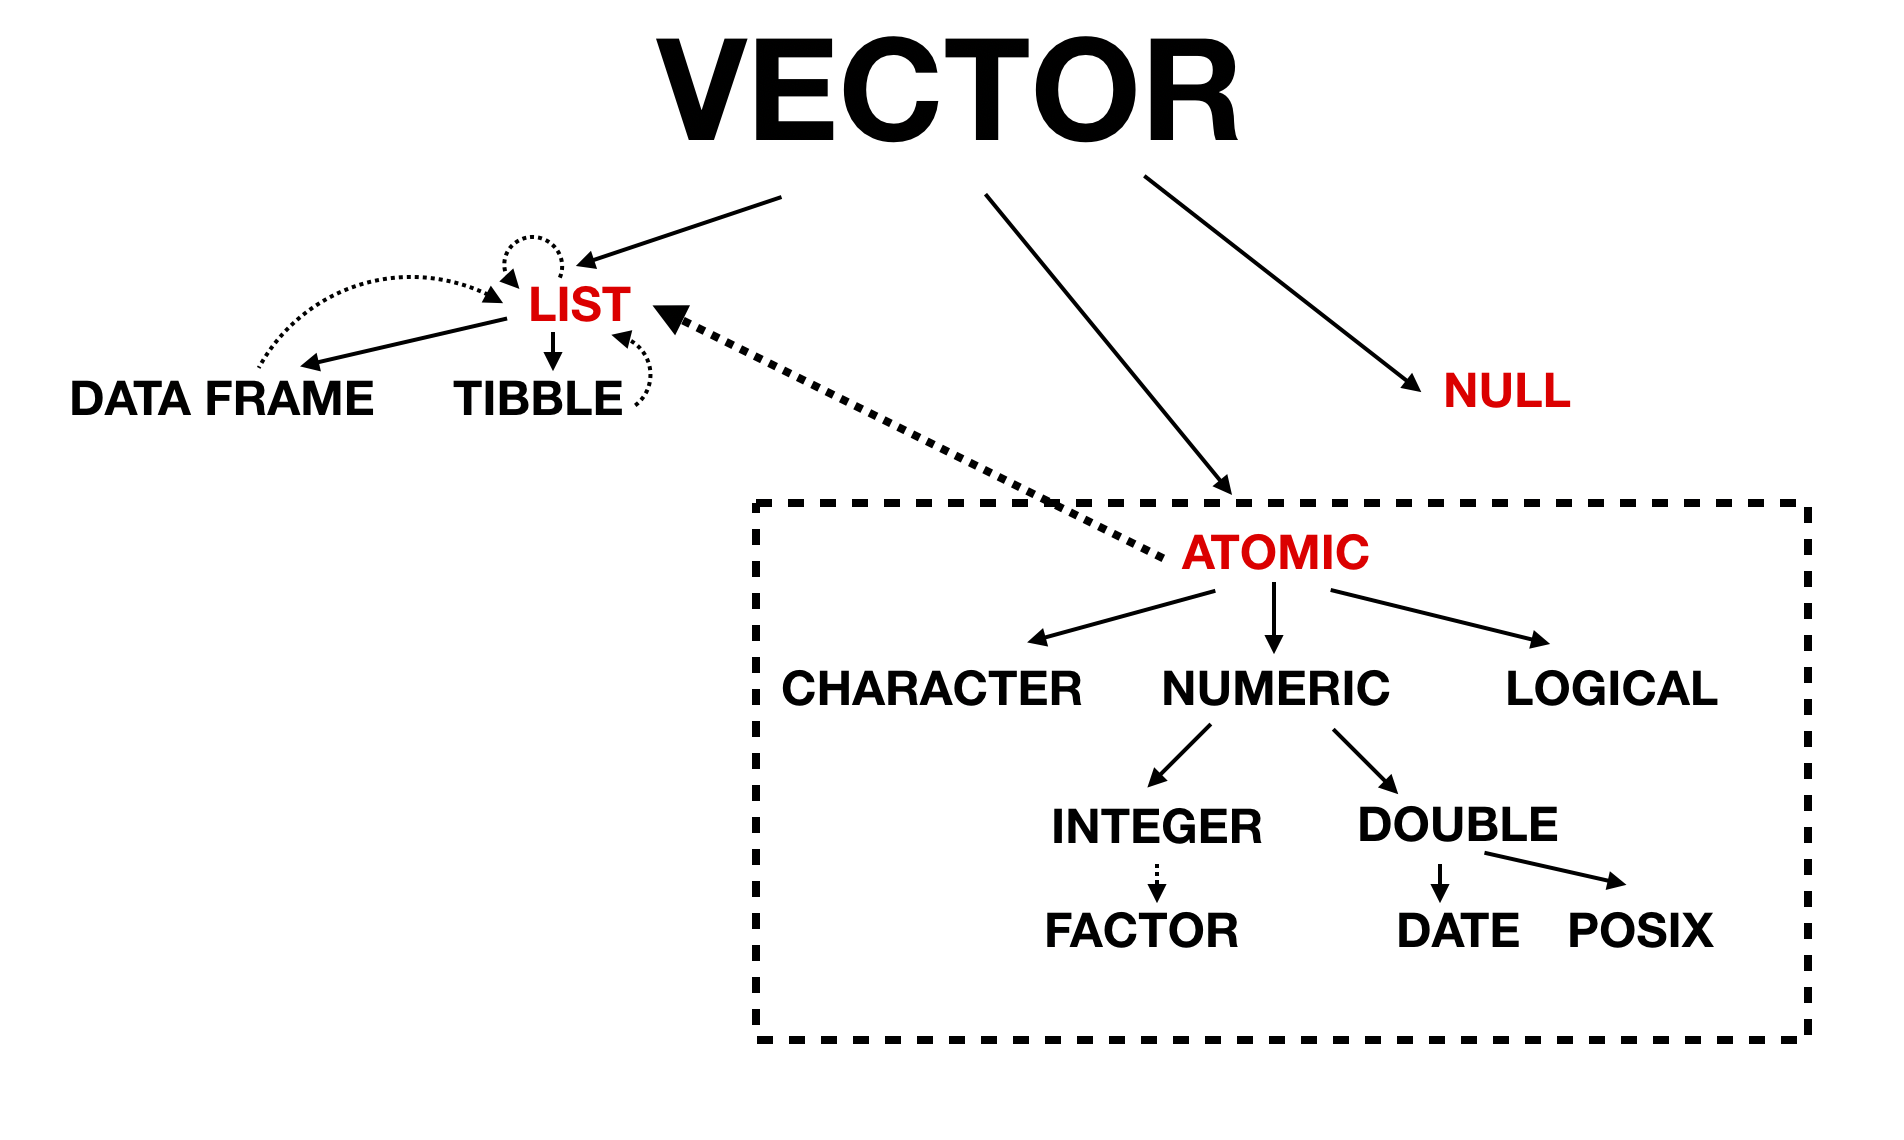
\includegraphics[width=26.44in]{images/vectors}

\hypertarget{subsetting}{%
\chapter{Subsetting}\label{subsetting}}

\hypertarget{introduction}{%
\section*{4.1 Introduction}\label{introduction}}
\addcontentsline{toc}{section}{4.1 Introduction}

"There are three subsetting operators \texttt{{[}}. \texttt{{[}{[}}, \texttt{\$}. What is the distinction between an operator and a function? When you look up the help page it brings up the same page for all three extraction methods. What are their distinctions and do their definitions change based on what you're subsetting? Can we make a table?

\hypertarget{selecting-multiple-elements}{%
\section*{4.2.1 Selecting multiple elements}\label{selecting-multiple-elements}}
\addcontentsline{toc}{section}{4.2.1 Selecting multiple elements}

Why is \texttt{numeric(0)} ``helpful for test data?''

This is more of a general comment that one should make sure one's code doesn't crash with vectors of zero length (or data frames with zero rows)

Why is subsetting with factors ``not a good idea''

Hadley's notes seem to say subsetting with factors uses the ``integer vector of levels'' - and if they all have the same level, it'll just return the first argument. Subsetting a factor vector leaves the factor levels behind unless you explicitly drop the unused levels

\hypertarget{lists_4}{%
\section*{4.2.2 lists}\label{lists_4}}
\addcontentsline{toc}{section}{4.2.2 lists}

We've been talking about \texttt{\$} as a shorthand for \texttt{{[}{[}}. Using the example list \texttt{x\ \textless{}-\ list(1:3,\ "a",\ 4:6)} can we use \texttt{x\$1} as shorthand for \texttt{x{[}{[}1{]}{]}}?

The ``shorthand'' refers to using the name of the vector to extract the vector. If we give \texttt{1:3} a name such as test = \texttt{1:3}

\begin{Shaded}
\begin{Highlighting}[]
\NormalTok{x <-}\StringTok{ }\KeywordTok{list}\NormalTok{(}\DataTypeTok{named_vector =} \DecValTok{1}\OperatorTok{:}\DecValTok{3}\NormalTok{, }\StringTok{"a"}\NormalTok{, }\DecValTok{4}\OperatorTok{:}\DecValTok{6}\NormalTok{)}
\NormalTok{x[[}\DecValTok{1}\NormalTok{]] }\OperatorTok{==}\StringTok{ }\NormalTok{x}\OperatorTok{$}\NormalTok{named_vector}
\end{Highlighting}
\end{Shaded}

\begin{verbatim}
## [1] TRUE TRUE TRUE
\end{verbatim}

As such, \texttt{\$} is a shorthand for \texttt{x{[}{[}"name\_of\_vector"{]}{]}} and not shorthand for \texttt{x{[}{[}index{]}{]}}

\hypertarget{subset_2}{%
\section*{\texorpdfstring{4.3.1 \texttt{{[}{[}}}{4.3.1 {[}{[}}}\label{subset_2}}
\addcontentsline{toc}{section}{4.3.1 \texttt{{[}{[}}}

The book states:

\emph{While you must use {[}{[} when working with lists, I'd also recommend using it with atomic vectors whenever you want to extract a single value. For example, instead of writing:}

\begin{Shaded}
\begin{Highlighting}[]
\ControlFlowTok{for}\NormalTok{ (i }\ControlFlowTok{in} \DecValTok{2}\OperatorTok{:}\KeywordTok{length}\NormalTok{(x)) \{}
\NormalTok{  out[i] <-}\StringTok{ }\KeywordTok{fun}\NormalTok{(x[i], out[i }\OperatorTok{-}\StringTok{ }\DecValTok{1}\NormalTok{])}
\NormalTok{\}}
\end{Highlighting}
\end{Shaded}

\emph{It's better to write}

\begin{Shaded}
\begin{Highlighting}[]
\ControlFlowTok{for}\NormalTok{ (i }\ControlFlowTok{in} \DecValTok{2}\OperatorTok{:}\KeywordTok{length}\NormalTok{(x)) \{}
\NormalTok{  out[[i]] <-}\StringTok{ }\KeywordTok{fun}\NormalTok{(x[[i]], out[[i }\OperatorTok{-}\StringTok{ }\DecValTok{1}\NormalTok{]])}
\NormalTok{\}}
\end{Highlighting}
\end{Shaded}

Why? Can we see this in action by giving \texttt{x}, \texttt{out}, and \texttt{fun} real life values?

If we have a vector

\begin{Shaded}
\begin{Highlighting}[]
\NormalTok{df_x <-}\StringTok{ }\KeywordTok{c}\NormalTok{(}\StringTok{"Advanced"}\NormalTok{,}\StringTok{"R"}\NormalTok{,}\StringTok{"Book"}\NormalTok{,}\StringTok{"Club"}\NormalTok{)}
\end{Highlighting}
\end{Shaded}

We can use \texttt{{[}} or \texttt{{[}{[}} to extract the third element of \texttt{df\_x}

\begin{Shaded}
\begin{Highlighting}[]
\NormalTok{df_x[}\DecValTok{3}\NormalTok{]}
\end{Highlighting}
\end{Shaded}

\begin{verbatim}
## [1] "Book"
\end{verbatim}

\begin{Shaded}
\begin{Highlighting}[]
\NormalTok{df_x[[}\DecValTok{3}\NormalTok{]]}
\end{Highlighting}
\end{Shaded}

\begin{verbatim}
## [1] "Book"
\end{verbatim}

But in the case where we want to extract an element from a list \texttt{{[}} and \texttt{{[}{[}} no longer give us the same results

\begin{Shaded}
\begin{Highlighting}[]
\NormalTok{df_x <-}\StringTok{ }\KeywordTok{list}\NormalTok{(}\DataTypeTok{A =} \StringTok{"Advanced"}\NormalTok{, }\DataTypeTok{B =} \StringTok{"R"}\NormalTok{, }\DataTypeTok{C =} \StringTok{"Book"}\NormalTok{, }\DataTypeTok{D =} \StringTok{"Club"}\NormalTok{)}

\NormalTok{df_x[}\DecValTok{3}\NormalTok{]}
\end{Highlighting}
\end{Shaded}

\begin{verbatim}
## $C
## [1] "Book"
\end{verbatim}

\begin{Shaded}
\begin{Highlighting}[]
\NormalTok{df_x[[}\DecValTok{3}\NormalTok{]]}
\end{Highlighting}
\end{Shaded}

\begin{verbatim}
## [1] "Book"
\end{verbatim}

Because using \texttt{{[}{[}} returns ``one element of this vector'' in both cases, it makes sense to default to \texttt{{[}{[}} instead of \texttt{{[}} since it will reliably return a single element.

\hypertarget{exercise_435}{%
\section*{4.3.5 Exercise}\label{exercise_435}}
\addcontentsline{toc}{section}{4.3.5 Exercise}

The question asks to describe the \texttt{upper.tri} function - let's dig into it!

\begin{Shaded}
\begin{Highlighting}[]
\NormalTok{x <-}\StringTok{ }\KeywordTok{outer}\NormalTok{(}\DecValTok{1}\OperatorTok{:}\DecValTok{5}\NormalTok{, }\DecValTok{1}\OperatorTok{:}\DecValTok{5}\NormalTok{, }\DataTypeTok{FUN =} \StringTok{"*"}\NormalTok{)}
\KeywordTok{upper.tri}\NormalTok{(x)}
\end{Highlighting}
\end{Shaded}

\begin{verbatim}
##       [,1]  [,2]  [,3]  [,4]  [,5]
## [1,] FALSE  TRUE  TRUE  TRUE  TRUE
## [2,] FALSE FALSE  TRUE  TRUE  TRUE
## [3,] FALSE FALSE FALSE  TRUE  TRUE
## [4,] FALSE FALSE FALSE FALSE  TRUE
## [5,] FALSE FALSE FALSE FALSE FALSE
\end{verbatim}

We see that it returns the upper triangle of the matrix. But I wanted to walk through how this function actually works and what is meant in the solution manual by leveraging \texttt{.row(dim(x))\ \textless{}=\ .col(dim(x))}.

\begin{Shaded}
\begin{Highlighting}[]
\CommentTok{# ?upper.tri}
\ControlFlowTok{function}\NormalTok{ (x, }\DataTypeTok{diag =} \OtherTok{FALSE}\NormalTok{) }
\NormalTok{\{}
\NormalTok{    d <-}\StringTok{ }\KeywordTok{dim}\NormalTok{(x)}
    \CommentTok{# if you have an array thats more than 2 dimension}
    \CommentTok{# we need to flatten it to a matrix}
    \ControlFlowTok{if}\NormalTok{ (}\KeywordTok{length}\NormalTok{(d) }\OperatorTok{!=}\StringTok{ }\NormalTok{2L) }
\NormalTok{        d <-}\StringTok{ }\KeywordTok{dim}\NormalTok{(}\KeywordTok{as.matrix}\NormalTok{(x))}
    \ControlFlowTok{if}\NormalTok{ (diag) }
      \CommentTok{# this is our subsetting logical!}
         \KeywordTok{.row}\NormalTok{(d) }\OperatorTok{<=}\StringTok{ }\KeywordTok{.col}\NormalTok{(d)}
    \ControlFlowTok{else} \KeywordTok{.row}\NormalTok{(d) }\OperatorTok{<}\StringTok{ }\KeywordTok{.col}\NormalTok{(d)}
\NormalTok{\}}
\end{Highlighting}
\end{Shaded}

The function \texttt{.row()} and \texttt{.col()} return a matrix of integers indicating their row number

\begin{Shaded}
\begin{Highlighting}[]
\KeywordTok{.row}\NormalTok{(}\KeywordTok{dim}\NormalTok{(x))}
\end{Highlighting}
\end{Shaded}

\begin{verbatim}
##      [,1] [,2] [,3] [,4] [,5]
## [1,]    1    1    1    1    1
## [2,]    2    2    2    2    2
## [3,]    3    3    3    3    3
## [4,]    4    4    4    4    4
## [5,]    5    5    5    5    5
\end{verbatim}

\begin{Shaded}
\begin{Highlighting}[]
\KeywordTok{.col}\NormalTok{(}\KeywordTok{dim}\NormalTok{(x))}
\end{Highlighting}
\end{Shaded}

\begin{verbatim}
##      [,1] [,2] [,3] [,4] [,5]
## [1,]    1    2    3    4    5
## [2,]    1    2    3    4    5
## [3,]    1    2    3    4    5
## [4,]    1    2    3    4    5
## [5,]    1    2    3    4    5
\end{verbatim}

\begin{Shaded}
\begin{Highlighting}[]
\KeywordTok{.row}\NormalTok{(}\KeywordTok{dim}\NormalTok{(x)) }\OperatorTok{<=}\StringTok{ }\KeywordTok{.col}\NormalTok{(}\KeywordTok{dim}\NormalTok{(x))}
\end{Highlighting}
\end{Shaded}

\begin{verbatim}
##       [,1]  [,2]  [,3]  [,4] [,5]
## [1,]  TRUE  TRUE  TRUE  TRUE TRUE
## [2,] FALSE  TRUE  TRUE  TRUE TRUE
## [3,] FALSE FALSE  TRUE  TRUE TRUE
## [4,] FALSE FALSE FALSE  TRUE TRUE
## [5,] FALSE FALSE FALSE FALSE TRUE
\end{verbatim}

Is there a high level meaning to a \texttt{.} before function? Does this refer to internal functions? {[}see: ?\texttt{row} vs ?\texttt{.row}{]}

Objects in the global environment prefixed with \texttt{.} are hidden in the R (and RStudio) environment panes - so functions prefixed as such are not visible unless you do \texttt{ls(all=TRUE)}. \href{https://community.rstudio.com/t/function-argument-naming-conventions-x-vs-x/7764}{Read more here} and (here){[}\url{https://stackoverflow.com/questions/7526467/what-does-the-dot-mean-in-r-personal-preference-naming-convention-or-more}{]}

\hypertarget{missing-and-oob}{%
\section*{4.3.3 Missing and OOB}\label{missing-and-oob}}
\addcontentsline{toc}{section}{4.3.3 Missing and OOB}

Let's walk through examples of each

\hypertarget{logical-atomic}{%
\subsection*{LOGICAL ATOMIC}\label{logical-atomic}}
\addcontentsline{toc}{subsection}{LOGICAL ATOMIC}

\begin{Shaded}
\begin{Highlighting}[]
\KeywordTok{c}\NormalTok{(}\OtherTok{TRUE}\NormalTok{, }\OtherTok{FALSE}\NormalTok{)[[}\DecValTok{0}\NormalTok{]] }\CommentTok{# zero length}
\CommentTok{# attempt to select less than one element in get1index <real>}
\KeywordTok{c}\NormalTok{(}\OtherTok{TRUE}\NormalTok{, }\OtherTok{FALSE}\NormalTok{)[[}\DecValTok{4}\NormalTok{]] }\CommentTok{# out of bounds}
\CommentTok{# subscript out of bounds}
\KeywordTok{c}\NormalTok{(}\OtherTok{TRUE}\NormalTok{, }\OtherTok{FALSE}\NormalTok{)[[}\OtherTok{NA}\NormalTok{]] }\CommentTok{# missing}
\CommentTok{# subscript out of bounds}
\end{Highlighting}
\end{Shaded}

\hypertarget{lists_missing}{%
\subsection*{LIST}\label{lists_missing}}
\addcontentsline{toc}{subsection}{LIST}

\begin{Shaded}
\begin{Highlighting}[]
\KeywordTok{list}\NormalTok{(}\DecValTok{1}\OperatorTok{:}\DecValTok{3}\NormalTok{, }\OtherTok{NULL}\NormalTok{)[[}\DecValTok{0}\NormalTok{]] }\CommentTok{# zero length}
\CommentTok{# attempt to select less than one element in get1index <real>}
\KeywordTok{list}\NormalTok{(}\DecValTok{1}\OperatorTok{:}\DecValTok{3}\NormalTok{, }\OtherTok{NULL}\NormalTok{)[[}\DecValTok{3}\NormalTok{]] }\CommentTok{# out of bounds}
\CommentTok{# subscript out of bounds}
\KeywordTok{list}\NormalTok{(}\DecValTok{1}\OperatorTok{:}\DecValTok{3}\NormalTok{, }\OtherTok{NULL}\NormalTok{)[[}\OtherTok{NA}\NormalTok{]] }\CommentTok{# missing}
\CommentTok{# NULL}
\end{Highlighting}
\end{Shaded}

\hypertarget{null}{%
\subsection*{NULL}\label{null}}
\addcontentsline{toc}{subsection}{NULL}

\begin{Shaded}
\begin{Highlighting}[]
\OtherTok{NULL}\NormalTok{[[}\DecValTok{0}\NormalTok{]] }\CommentTok{# zero length}
\CommentTok{# NULL}
\OtherTok{NULL}\NormalTok{[[}\DecValTok{1}\NormalTok{]] }\CommentTok{# out of bounds}
\CommentTok{# NULL}
\OtherTok{NULL}\NormalTok{[[}\OtherTok{NA}\NormalTok{]] }\CommentTok{# missing}
\CommentTok{# NULL}
\end{Highlighting}
\end{Shaded}

\hypertarget{logical-subsetting}{%
\section*{4.5.8 Logical subsetting}\label{logical-subsetting}}
\addcontentsline{toc}{section}{4.5.8 Logical subsetting}

``Remember to use the vector Boolean operators \texttt{\&} and \texttt{\textbar{}}, not the short-circuiting scalar operators \texttt{\&\&} and \texttt{\textbar{}\textbar{}}, which are more useful inside if statements.''

Can we go over the difference between \texttt{\&} and \texttt{\&\&} (and \texttt{\textbar{}} vs \texttt{\textbar{}\textbar{}}) I use brute force to figure out which ones I need\ldots{}

\texttt{\&\&} and \texttt{\textbar{}\textbar{}} only ever return a single (scalar, length-1 vector) \texttt{TRUE} or \texttt{FALSE} value, whereas \texttt{\textbar{}} and \texttt{\&} return a vector after doing element-by-element comparisons.

The only place in R you routinely use a scalar \texttt{TRUE}/\texttt{FALSE} value is in the conditional of an \texttt{if} statement, so you'll often see \texttt{\&\&} or \texttt{\textbar{}\textbar{}} used in idioms like: \texttt{if\ (length(x)\ \textgreater{}\ 0\ \&\&\ any(is.na(x)))\ \{\ do.something()\ \}}

In most other instances you'll be working with vectors and use \texttt{\&} and \texttt{\textbar{}} instead.

Using \texttt{\&\&} or \texttt{\textbar{}\textbar{}} results in some unexpected behavior - which could be a big performance gain in some cases:

\begin{itemize}
\tightlist
\item
  \texttt{\textbar{}\textbar{}} will not evaluate the second argument when the first is \texttt{TRUE}
\item
  \texttt{\&\&} will not evaluate the second argument when the first is \texttt{FALSE}
\end{itemize}

\begin{Shaded}
\begin{Highlighting}[]
\NormalTok{true_one <-}\StringTok{ }\ControlFlowTok{function}\NormalTok{() \{ }\KeywordTok{print}\NormalTok{(}\StringTok{"true_one evaluated."}\NormalTok{); }\OtherTok{TRUE}\NormalTok{\}}
\NormalTok{true_two <-}\StringTok{ }\ControlFlowTok{function}\NormalTok{() \{ }\KeywordTok{print}\NormalTok{(}\StringTok{"true_two evaluated."}\NormalTok{); }\OtherTok{TRUE}\NormalTok{\}}
\CommentTok{# arguments are evaluated lazily.  Unexpected behavior can result:}
\KeywordTok{c}\NormalTok{(T, }\KeywordTok{true_one}\NormalTok{()) }\OperatorTok{&&}\StringTok{ }\KeywordTok{c}\NormalTok{(T, }\KeywordTok{true_two}\NormalTok{())}
\end{Highlighting}
\end{Shaded}

\begin{verbatim}
## [1] "true_one evaluated."
## [1] "true_two evaluated."
\end{verbatim}

\begin{verbatim}
## [1] TRUE
\end{verbatim}

\begin{Shaded}
\begin{Highlighting}[]
\KeywordTok{c}\NormalTok{(T, }\KeywordTok{true_one}\NormalTok{()) }\OperatorTok{&&}\StringTok{ }\KeywordTok{c}\NormalTok{(F, }\KeywordTok{true_two}\NormalTok{())}
\end{Highlighting}
\end{Shaded}

\begin{verbatim}
## [1] "true_one evaluated."
## [1] "true_two evaluated."
\end{verbatim}

\begin{verbatim}
## [1] FALSE
\end{verbatim}

\begin{Shaded}
\begin{Highlighting}[]
\KeywordTok{c}\NormalTok{(F, }\KeywordTok{true_one}\NormalTok{()) }\OperatorTok{&&}\StringTok{ }\KeywordTok{c}\NormalTok{(T, }\KeywordTok{true_two}\NormalTok{()) }
\end{Highlighting}
\end{Shaded}

\begin{verbatim}
## [1] "true_one evaluated."
\end{verbatim}

\begin{verbatim}
## [1] FALSE
\end{verbatim}

\begin{Shaded}
\begin{Highlighting}[]
\KeywordTok{c}\NormalTok{(F, }\KeywordTok{true_one}\NormalTok{()) }\OperatorTok{&&}\StringTok{ }\KeywordTok{c}\NormalTok{(F, }\KeywordTok{true_two}\NormalTok{()) }
\end{Highlighting}
\end{Shaded}

\begin{verbatim}
## [1] "true_one evaluated."
\end{verbatim}

\begin{verbatim}
## [1] FALSE
\end{verbatim}

\begin{Shaded}
\begin{Highlighting}[]
\KeywordTok{c}\NormalTok{(T, }\KeywordTok{true_one}\NormalTok{()) }\OperatorTok{||}\StringTok{ }\KeywordTok{c}\NormalTok{(T, }\KeywordTok{true_two}\NormalTok{())}
\end{Highlighting}
\end{Shaded}

\begin{verbatim}
## [1] "true_one evaluated."
\end{verbatim}

\begin{verbatim}
## [1] TRUE
\end{verbatim}

\begin{Shaded}
\begin{Highlighting}[]
\KeywordTok{c}\NormalTok{(T, }\KeywordTok{true_one}\NormalTok{()) }\OperatorTok{||}\StringTok{ }\KeywordTok{c}\NormalTok{(F, }\KeywordTok{true_two}\NormalTok{())}
\end{Highlighting}
\end{Shaded}

\begin{verbatim}
## [1] "true_one evaluated."
\end{verbatim}

\begin{verbatim}
## [1] TRUE
\end{verbatim}

\begin{Shaded}
\begin{Highlighting}[]
\KeywordTok{c}\NormalTok{(F, }\KeywordTok{true_one}\NormalTok{()) }\OperatorTok{||}\StringTok{ }\KeywordTok{c}\NormalTok{(T, }\KeywordTok{true_two}\NormalTok{()) }
\end{Highlighting}
\end{Shaded}

\begin{verbatim}
## [1] "true_one evaluated."
## [1] "true_two evaluated."
\end{verbatim}

\begin{verbatim}
## [1] TRUE
\end{verbatim}

\begin{Shaded}
\begin{Highlighting}[]
\KeywordTok{c}\NormalTok{(F, }\KeywordTok{true_one}\NormalTok{()) }\OperatorTok{||}\StringTok{ }\KeywordTok{c}\NormalTok{(F, }\KeywordTok{true_two}\NormalTok{()) }
\end{Highlighting}
\end{Shaded}

\begin{verbatim}
## [1] "true_one evaluated."
## [1] "true_two evaluated."
\end{verbatim}

\begin{verbatim}
## [1] FALSE
\end{verbatim}

Read more about \href{https://cran.r-project.org/doc/manuals/r-release/R-ints.html\#Special-primitives}{Special Primatives} here

\hypertarget{boolean-algebra}{%
\section*{4.5.8 Boolean algebra}\label{boolean-algebra}}
\addcontentsline{toc}{section}{4.5.8 Boolean algebra}

The \texttt{unwhich()} function takes a boolean and turns it into a numeric - would this ever be useful? How?

XXX

``\texttt{x{[}-which(y){]}} is not equivalent to \texttt{x{[}!y{]}}: if \texttt{y} is all FALSE, \texttt{which(y)} will be \texttt{integer(0)} and \texttt{-integer(0)} is still \texttt{integer(0)}, so you'll get no values, instead of all values.''

Can we come up with an example for this plugging in values for \texttt{x} and \texttt{y}

\begin{Shaded}
\begin{Highlighting}[]
\KeywordTok{c}\NormalTok{(}\OtherTok{TRUE}\NormalTok{, }\OtherTok{FALSE}\NormalTok{)[}\OperatorTok{-}\KeywordTok{which}\NormalTok{(}\OtherTok{FALSE}\NormalTok{)]}
\end{Highlighting}
\end{Shaded}

\begin{verbatim}
## logical(0)
\end{verbatim}

\begin{Shaded}
\begin{Highlighting}[]
\KeywordTok{c}\NormalTok{(}\OtherTok{TRUE}\NormalTok{, }\OtherTok{FALSE}\NormalTok{)[}\OperatorTok{!}\OtherTok{FALSE}\NormalTok{]}
\end{Highlighting}
\end{Shaded}

\begin{verbatim}
## [1]  TRUE FALSE
\end{verbatim}

\hypertarget{control-flow}{%
\chapter{Control Flow}\label{control-flow}}

\hypertarget{vectorised-if}{%
\section*{5.2.2 Vectorised if}\label{vectorised-if}}
\addcontentsline{toc}{section}{5.2.2 Vectorised if}

Why does \texttt{if} \texttt{else} print \texttt{"Out\ of\ range"} once but \texttt{ifelse} prints it twice?

\begin{Shaded}
\begin{Highlighting}[]
\ControlFlowTok{if}\NormalTok{ (}\KeywordTok{sample}\NormalTok{(}\DecValTok{1}\OperatorTok{:}\DecValTok{10}\NormalTok{, }\DecValTok{1}\NormalTok{) }\OperatorTok{==}\StringTok{ }\DecValTok{1}\NormalTok{) }\KeywordTok{print}\NormalTok{(}\StringTok{"In range"}\NormalTok{) }\ControlFlowTok{else} \KeywordTok{print}\NormalTok{(}\StringTok{"Out of range"}\NormalTok{)}
\end{Highlighting}
\end{Shaded}

\begin{verbatim}
[1] "Out of range"
\end{verbatim}

\begin{Shaded}
\begin{Highlighting}[]
\KeywordTok{ifelse}\NormalTok{((}\KeywordTok{sample}\NormalTok{(}\DecValTok{1}\OperatorTok{:}\DecValTok{10}\NormalTok{, }\DecValTok{1}\NormalTok{) }\OperatorTok{==}\StringTok{ }\DecValTok{1}\NormalTok{), }\KeywordTok{print}\NormalTok{(}\StringTok{"In range"}\NormalTok{), }\KeywordTok{print}\NormalTok{(}\StringTok{"Out of range"}\NormalTok{))}
\end{Highlighting}
\end{Shaded}

\begin{verbatim}
[1] "Out of range"
[1] "Out of range"
\end{verbatim}

\begin{Shaded}
\begin{Highlighting}[]
\NormalTok{var <-}\StringTok{ }\ControlFlowTok{if}\NormalTok{ (}\KeywordTok{sample}\NormalTok{(}\DecValTok{1}\OperatorTok{:}\DecValTok{10}\NormalTok{, }\DecValTok{1}\NormalTok{) }\OperatorTok{==}\StringTok{ }\DecValTok{1}\NormalTok{) }\KeywordTok{print}\NormalTok{(}\StringTok{"In range"}\NormalTok{)}
\NormalTok{var}
\end{Highlighting}
\end{Shaded}

\begin{verbatim}
NULL
\end{verbatim}

\begin{Shaded}
\begin{Highlighting}[]
\NormalTok{var <-}\StringTok{ }\KeywordTok{ifelse}\NormalTok{((}\KeywordTok{sample}\NormalTok{(}\DecValTok{1}\OperatorTok{:}\DecValTok{10}\NormalTok{, }\DecValTok{1}\NormalTok{) }\OperatorTok{==}\StringTok{ }\DecValTok{1}\NormalTok{), }\KeywordTok{print}\NormalTok{(}\StringTok{"In range"}\NormalTok{), }\KeywordTok{print}\NormalTok{(}\StringTok{"Out of range"}\NormalTok{))}
\end{Highlighting}
\end{Shaded}

\begin{verbatim}
## [1] "Out of range"
\end{verbatim}

\begin{Shaded}
\begin{Highlighting}[]
\NormalTok{var}
\end{Highlighting}
\end{Shaded}

\begin{verbatim}
## [1] "Out of range"
\end{verbatim}

\texttt{ifelse} explicitly returns its result, whereas \texttt{if} invisibly returns it!

\hypertarget{loops}{%
\section*{5.3 Loops}\label{loops}}
\addcontentsline{toc}{section}{5.3 Loops}

Can the body of the loop change the set?

\begin{Shaded}
\begin{Highlighting}[]
\NormalTok{my_set <-}\StringTok{ }\KeywordTok{c}\NormalTok{(}\DecValTok{1}\NormalTok{, }\DecValTok{20}\NormalTok{, }\DecValTok{99}\NormalTok{)}

\ControlFlowTok{for}\NormalTok{ (i }\ControlFlowTok{in}\NormalTok{ my_set)\{}
  \ControlFlowTok{if}\NormalTok{ (i}\OperatorTok{==}\DecValTok{1}\NormalTok{)\{}
\NormalTok{    my_set[}\DecValTok{9}\NormalTok{]=}\StringTok{ }\DecValTok{20}
\NormalTok{    \}}
  \KeywordTok{print}\NormalTok{(}\StringTok{"hello"}\NormalTok{)}
  \KeywordTok{print}\NormalTok{(my_set)}
\NormalTok{  \}}
\end{Highlighting}
\end{Shaded}

\begin{verbatim}
## [1] "hello"
## [1]  1 20 99 NA NA NA NA NA 20
## [1] "hello"
## [1]  1 20 99 NA NA NA NA NA 20
## [1] "hello"
## [1]  1 20 99 NA NA NA NA NA 20
\end{verbatim}

Looks like you can't!

\hypertarget{switch}{%
\section*{5.2.3 switch statement}\label{switch}}
\addcontentsline{toc}{section}{5.2.3 switch statement}

``Closely related to if is the \texttt{switch()} statement. It's a compact, special purpose equivalent''

What is meant here by ``special purpose''? Can we come up with a case where you can't substitute \texttt{if} for \texttt{switch} or the other way around? Use \texttt{switch}. Is it safe to say to \texttt{switch} when you have character inputs (as the book suggests) and use \texttt{case\_when} or \texttt{if} for numerics?

Switch is special in that only ONE value can be true, as in the case from our presentation the shiny input can only ever be ONE of the strings on the left it cannot be multiple.

\begin{Shaded}
\begin{Highlighting}[]
\NormalTok{datasetInput <-}\StringTok{ }\KeywordTok{reactive}\NormalTok{(\{ }
  \ControlFlowTok{switch}\NormalTok{(input}\OperatorTok{$}\NormalTok{dataset,}
         \StringTok{"materials"}\NormalTok{ =}\StringTok{ }\NormalTok{brewing_materials,}
         \StringTok{"size"}\NormalTok{ =}\StringTok{ }\NormalTok{brewer_size,}
         \StringTok{"states"}\NormalTok{ =}\StringTok{ }\NormalTok{beer_states,}
         \StringTok{"taxed"}\NormalTok{ =}\StringTok{ }\NormalTok{beer_taxed)}
\NormalTok{\})}
\end{Highlighting}
\end{Shaded}

\hypertarget{common-pitfalls}{%
\section*{5.3.1 common pitfalls}\label{common-pitfalls}}
\addcontentsline{toc}{section}{5.3.1 common pitfalls}

What does the book mean by leveraging \texttt{vector} for preallocating the loop output? How is this different from creating an empty list to instantiate the loop?

\begin{Shaded}
\begin{Highlighting}[]
\NormalTok{means <-}\StringTok{ }\KeywordTok{c}\NormalTok{(}\DecValTok{1}\NormalTok{, }\DecValTok{50}\NormalTok{, }\DecValTok{20}\NormalTok{)}

\NormalTok{out_vector <-}\StringTok{ }\KeywordTok{vector}\NormalTok{(}\StringTok{"list"}\NormalTok{, }\KeywordTok{length}\NormalTok{(means))}
\ControlFlowTok{for}\NormalTok{ (i }\ControlFlowTok{in} \DecValTok{1}\OperatorTok{:}\KeywordTok{length}\NormalTok{(means)) \{}
\NormalTok{  out_vector[[i]] <-}\StringTok{ }\KeywordTok{rnorm}\NormalTok{(}\DecValTok{10}\NormalTok{, means[[i]])}
\NormalTok{\}}

\NormalTok{out_list <-}\StringTok{ }\KeywordTok{list}\NormalTok{()}
\ControlFlowTok{for}\NormalTok{ (i }\ControlFlowTok{in} \DecValTok{1}\OperatorTok{:}\KeywordTok{length}\NormalTok{(means)) \{}
\NormalTok{  out_list[[i]] <-}\StringTok{ }\KeywordTok{rnorm}\NormalTok{(}\DecValTok{10}\NormalTok{, means[[i]])}
\NormalTok{\}}
\end{Highlighting}
\end{Shaded}

By preallocating the length of the \texttt{out\_vector} we're leveraging \texttt{modify-in-place} rather than \texttt{copy-on-modify}.

The book warns against using \texttt{length(x)} and suggests using \texttt{seq\_along} instead. Is there any downside to using \texttt{seq\_along} or a case when you'd prefer \texttt{length(x)} over \texttt{seq\_along(x)}? I can't think of any downsides to using it!

We have yet to find a downside but should look into this further!

\hypertarget{exercise5331}{%
\section*{5.3.3.1 Exercises}\label{exercise5331}}
\addcontentsline{toc}{section}{5.3.3.1 Exercises}

\begin{Shaded}
\begin{Highlighting}[]
\NormalTok{x <-}\StringTok{ }\KeywordTok{numeric}\NormalTok{()}
\NormalTok{out <-}\StringTok{ }\KeywordTok{vector}\NormalTok{(}\StringTok{"list"}\NormalTok{, }\KeywordTok{length}\NormalTok{(x))}
\ControlFlowTok{for}\NormalTok{ (i }\ControlFlowTok{in} \DecValTok{1}\OperatorTok{:}\KeywordTok{length}\NormalTok{(x)) \{}
\NormalTok{  out[i] <-}\StringTok{ }\NormalTok{x[i] }\OperatorTok{^}\StringTok{ }\DecValTok{2}
\NormalTok{\}}
\NormalTok{out}
\end{Highlighting}
\end{Shaded}

\begin{verbatim}
## [[1]]
## [1] NA
\end{verbatim}

I understand that this works because we can count down in a loop - so the first iteration \texttt{x{[}1{]}\ ==\ NA}, and the second \texttt{x{[}2{]}\ ==\ numeric(0)} but where does this value go? Is it just evaluated but not stored since R counts from 1?

This question is actually the bigger question, ``Can you assign something to index 0 in R?'' and it doesn't seem that you can.

\hypertarget{assignment-valid}{%
\subsection*{Assignment to a valid index}\label{assignment-valid}}
\addcontentsline{toc}{subsection}{Assignment to a valid index}

\begin{Shaded}
\begin{Highlighting}[]
\NormalTok{mylist =}\StringTok{ }\KeywordTok{list}\NormalTok{()}
\NormalTok{mylist[}\DecValTok{1}\NormalTok{] <-}\StringTok{ }\KeywordTok{c}\NormalTok{(}\StringTok{"something"}\NormalTok{)}
\NormalTok{mylist[}\DecValTok{1}\NormalTok{]}
\end{Highlighting}
\end{Shaded}

\begin{verbatim}
## [[1]]
## [1] "something"
\end{verbatim}

\hypertarget{assignment-0}{%
\subsection*{Assignment to {[}0{]}}\label{assignment-0}}
\addcontentsline{toc}{subsection}{Assignment to {[}0{]}}

\begin{Shaded}
\begin{Highlighting}[]
\NormalTok{mylist =}\StringTok{ }\KeywordTok{list}\NormalTok{()}
\NormalTok{mylist[}\DecValTok{0}\NormalTok{] <-}\StringTok{ }\KeywordTok{c}\NormalTok{(}\StringTok{"something"}\NormalTok{)}
\NormalTok{mylist[}\DecValTok{0}\NormalTok{]}
\end{Highlighting}
\end{Shaded}

\begin{verbatim}
## list()
\end{verbatim}

It's interesting that it's syntactically correct to assign to \texttt{mylist{[}0{]}} but it does nothing!

\hypertarget{empty-index}{%
\subsection*{Empty index}\label{empty-index}}
\addcontentsline{toc}{subsection}{Empty index}

\begin{Shaded}
\begin{Highlighting}[]
\NormalTok{mylist =}\StringTok{ }\KeywordTok{list}\NormalTok{()}
\NormalTok{mylist[}\DecValTok{1}\NormalTok{]}
\end{Highlighting}
\end{Shaded}

\begin{verbatim}
## [[1]]
## NULL
\end{verbatim}

R defaultly accesses the first layer using \texttt{{[}} and says there are no elements in the first layer of \texttt{mylist} and returns \texttt{NULL}. But when you do \texttt{mylist{[}{[}1{]}{]}} R says \texttt{Out\ of\ Bounds} because the first layer of \texttt{mylist} has been called and there is no layer at all. That's why R throws error in \texttt{{[}{[}} case.

\hypertarget{impossible-double}{%
\subsection*{\texorpdfstring{Impossible Index \texttt{{[}{[}}}{Impossible Index {[}{[}}}\label{impossible-double}}
\addcontentsline{toc}{subsection}{Impossible Index \texttt{{[}{[}}}

\begin{Shaded}
\begin{Highlighting}[]
\NormalTok{mylist =}\StringTok{ }\KeywordTok{list}\NormalTok{()}
\NormalTok{mylist[[}\DecValTok{0}\NormalTok{]]}
\end{Highlighting}
\end{Shaded}

\begin{verbatim}
Error in mylist[[0]] : attempt to select less than one element in get1index <real>
\end{verbatim}

\texttt{{[}{[}} isolates one element whereas \texttt{{[}} can be used to get subsets of varying sizes.
\texttt{{[}{[}} gets precisely one element, no more no less, or it fails. So \texttt{{[}{[}0{]}{]}\textless{}-} cannot work because index zero cannot hold a value.

\hypertarget{impossible-double-assign}{%
\subsection*{\texorpdfstring{Impossible Index \texttt{{[}{[}\textless{}-}}{Impossible Index {[}{[}\textless{}-}}\label{impossible-double-assign}}
\addcontentsline{toc}{subsection}{Impossible Index \texttt{{[}{[}\textless{}-}}

\begin{Shaded}
\begin{Highlighting}[]
\NormalTok{mylist =}\StringTok{ }\KeywordTok{list}\NormalTok{()}
\NormalTok{mylist[[}\DecValTok{0}\NormalTok{]] <-}\StringTok{ "something"}
\end{Highlighting}
\end{Shaded}

\begin{verbatim}
Error in mylist[[0]] <- "something" : attempt to select less than one element in integerOneIndex
\end{verbatim}

\hypertarget{undefined-5}{%
\subsection*{Undefined name}\label{undefined-5}}
\addcontentsline{toc}{subsection}{Undefined name}

Selection using an undefined - but possible name - gives NULL

\begin{Shaded}
\begin{Highlighting}[]
\NormalTok{mylist =}\StringTok{ }\KeywordTok{list}\NormalTok{()}
\NormalTok{mylist[[}\StringTok{"undefined_name"}\NormalTok{]]}
\end{Highlighting}
\end{Shaded}

\hypertarget{oob-5}{%
\subsection*{Out of Bounds}\label{oob-5}}
\addcontentsline{toc}{subsection}{Out of Bounds}

Selection using a possible - but not currently allocated - index gives an out of bounds error

\begin{Shaded}
\begin{Highlighting}[]
\NormalTok{mylist =}\StringTok{ }\KeywordTok{list}\NormalTok{()}
\NormalTok{mylist[[}\DecValTok{10}\NormalTok{]]}
\end{Highlighting}
\end{Shaded}

\begin{verbatim}
Error in mylist[[10]] : subscript out of bounds 
\end{verbatim}

\hypertarget{conclusion-5}{%
\section*{Conclusion}\label{conclusion-5}}
\addcontentsline{toc}{section}{Conclusion}

Can we put these concepts together in diagram form? Let's work on improving these schematics!

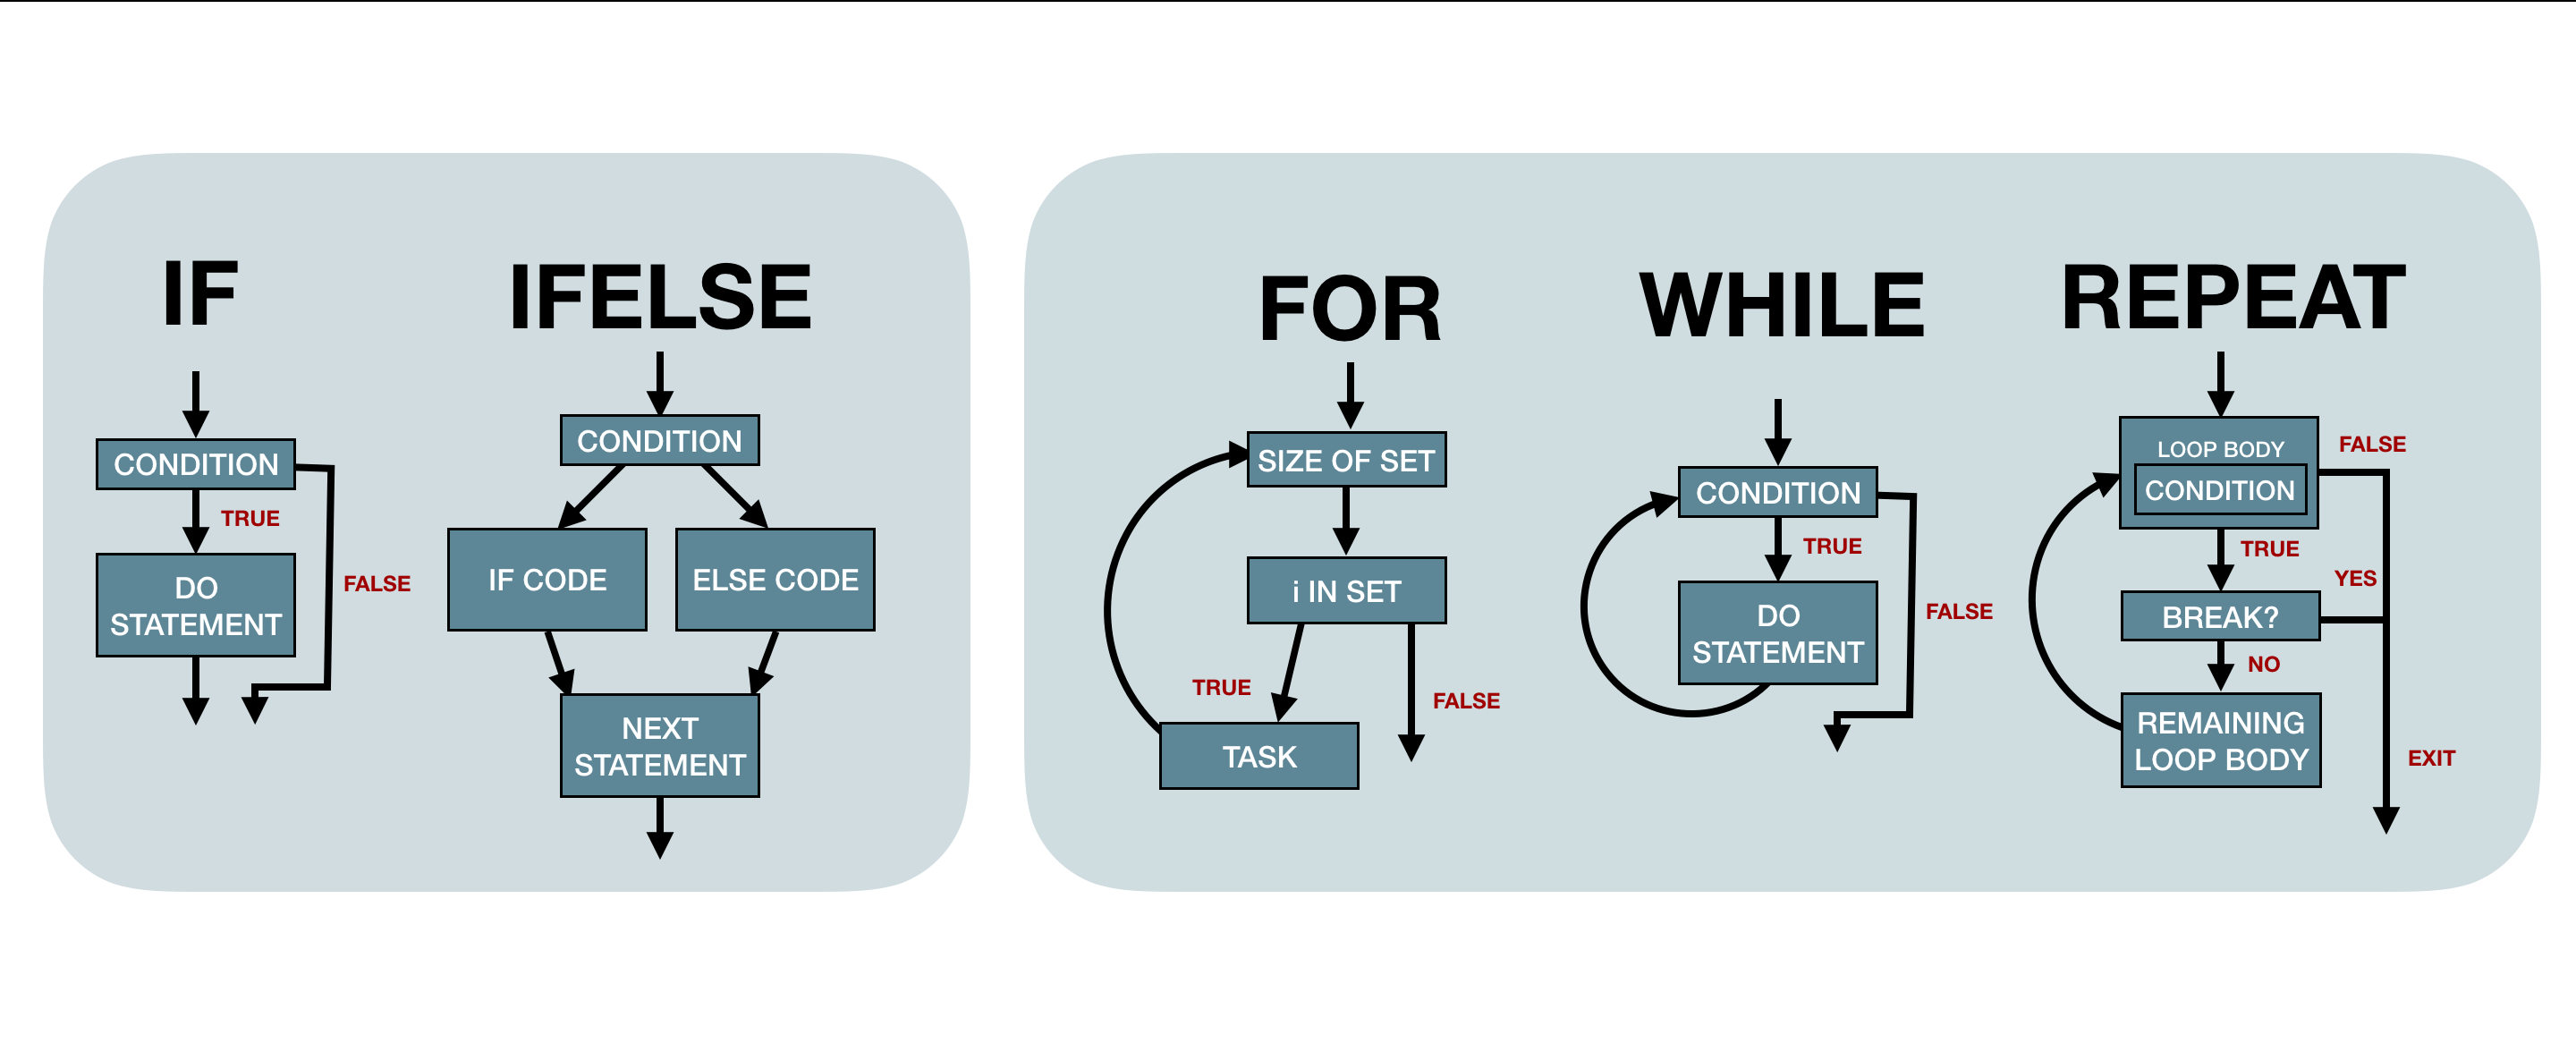
\includegraphics[width=40in]{images/controlflow}

\bibliography{book.bib,packages.bib}

\end{document}
